% This is samplepaper.tex, a sample chapter demonstrating the
% LLNCS macro package for Springer Computer Science proceedings;
% Version 2.20 of 2017/10/04
%
\documentclass[runningheads]{llncs}
%
\usepackage{graphicx}
\usepackage{algorithmic}
\usepackage{threeparttable}
\usepackage{caption}
% \usepackage{subfigure}
% \usepackage{amsthm}
\usepackage{amsmath, amssymb,amsfonts}
\usepackage{textcomp}
\usepackage{subcaption}
\usepackage{textcomp}
\usepackage{xcolor}
\usepackage{hyperref}
\usepackage[lined,boxed,commentsnumbered,ruled,vlined,linesnumbered]{algorithm2e}
\usepackage{amsfonts}
\usepackage{marvosym}
\usepackage{array}
\newcolumntype{P}[1]{>{\centering\arraybackslash}p{#1}}
% \usepackage{titling}

\newtheorem{defi}{Definition}
\DeclareMathOperator*{\argmin}{argmin}
\DeclareMathOperator*{\argmax}{argmax}

% Used for displaying a sample figure. If possible, figure files should
% be included in EPS format.
%
% If you use the hyperref package, please uncomment the following line
% to display URLs in blue roman font according to Springer's eBook style:
% \renewcommand\UrlFont{\color{blue}\rmfamily}
\title{HEM: A Hardware-aware Event Matching Algorithm for Content-based Pub/Sub Systems}
% \titlerunning{HEM: A Hardware-aware Event Matching Algorithm }
% \author{\vspace{-5ex}}
% \institute{\vspace{-5ex}}
% \date{}
\begin{document}
%
% \title{Contribution Title\thanks{Supported by organization x.}}

\titlerunning{HEM: A Hardware-aware Event Matching Algorithm}
% If the paper title is too long for the running head, you can set
% an abbreviated paper title here
% \inst{1}\orcidID{0000-1111-2222-3333}
\author{Wanghua Shi \and Shiyou Qian$\textsuperscript{(\Letter)}$}
% %
\authorrunning{W. Shi \and S. Qian}
% First names are abbreviated in the running head.
% If there are more than two authors, 'et al.' is used.
%
\institute{Shanghai Jiao Tong University, Shanghai, China\\
\email{s-whua@sjtu.edu.cn}, 
\email{qshiyou@sjtu.edu.cn}}
% \institute{Princeton University, Princeton NJ 08544, USA \and
% Springer Heidelberg, Tiergartenstr. 17, 69121 Heidelberg, Germany
% \email{lncs@springer.com}\\
% \url{http://www.springer.com/gp/computer-science/lncs} \and
% ABC Institute, Rupert-Karls-University Heidelberg, Heidelberg, Germany\\
% \email{\{abc,lncs\}@uni-heidelberg.de}}
%
\maketitle              % typeset the header of the contribution
%
% \begin{abstract}
% The abstract should briefly summarize the contents of the paper in
% 15--250 words.

% \keywords{First keyword  \and Second keyword \and Another keyword.}
% \end{abstract}
\begin{abstract}
Content-based publish/subscribe (CPS) systems are widely used in many fields to achieve selective data distribution. Event matching is a key component in the CPS system. Many efficient algorithms have been proposed to improve matching performance. However, most of the existing work seldom considers the hardware characteristics, resulting in performance degradation due to a large number of repetitive operations, such as comparison, addition and assignment. In this paper, we propose a Hardware-aware Event Matching algorithm called HEM. The basic idea behind HEM is that we perform as many bit OR operations as possible during the matching process, which is most efficient for the hardware. In addition, we build a performance analysis model that quantifies the trade-off between memory consumption and performance improvement. We conducted extensive experiments to evaluate the performance of HEM. On average, HEM reduces matching time by up to 86.8\% compared with the counterparts. 
%  The 7-day experimental results on the Manhattan dataset show that @Me can carry an additional 48,332 passengers and increase drivers' revenue by \$570,317.

% Taxi, route recommendation, demand prediction, force model, balance.

\keywords{Event matching \and Hardware-aware  \and Bitset OR operation.}
\end{abstract}

% Pages: abstract + introduction: 2;  related work: 1; design:7 pages; experiment:5 reference: 1;

\section{Introduction}
\label{intro}
As a flexible communication paradigm, content-based publish/subscribe (CPS) systems are widely applied in manifold applications, such as stock trading system \cite{2010Efficient} \cite{2014Elastic}, recommendation system \cite{2010Efficiently}, social message dissemination system \cite{2020Topk} and monitoring system \cite{A-Tree}. There are three basic roles in CPS systems to achieve fine-grained data distribution: subscriber, publisher and broker. Subscribers commit subscriptions to brokers according to their interests and focuses. Publishers produce events and send them to brokers. For each incoming event, brokers execute event matching algorithms to search for matching subscriptions and forward the event to the subscribers to which those matches belong.

Apparently, matching algorithms play an irreplaceable role in CPS systems. With the growth of event arrival rate, subscription number and the size of event and subscription, it is inevitable for event matching algorithm to be a performance bottleneck of the entire CPS system. The urge to decrease the end-to-end data distribution latency and improve the throughput in CPS systems in the past decades has driven algorithm design in event matching.

Diverse algorithms have been proposed to boost event matching. According to the first search targets (matching or unmatching subscriptions), there are forward algorithms (such as TAMA \cite{TAMA} and OpIndex \cite{OpIndex}) and backward algorithms (such as REIN \cite{REIN} and GEM \cite{GEM}). 
Each matching algorithm has its own design idea. For example,
TAMA \cite{TAMA} designs an index table to locate all the predicates matching a given event value and maintains a counter for each subscription. REIN \cite{REIN} locates two unmatching cell lists for each event value and traverses the cells to mark unmatching subscriptions. 
From the hardware perspective, TAMA and OpIndex do numerous addition operations one by one while REIN and GEM perform arduous traversal and marking operations bit by bit, thereby consuming much time to do repetitive operations. In effect, it is more efficient for computers to do in-flash bitwise operations because the overhead of data movement between caches and memory is mitigated \cite{ParaBit}. In addition, as the memory price is falling and large capacity of memory becomes more common nowadays, cache mechanism becomes a potential method to trade space for time.

% task load prediction
Motivated by the above discussion, we propose a novel hardware-aware event matching algorithm (HEM) based on bitset OR operations. 
HEM adopts a backward method to obtain matching results, similar to REIN \cite{REIN} and GEM \cite{GEM}.
The basic idea is to fully utilize the hardware characteristic of doing a set of bitwise OR operations in the parallel way. 
Specifically, HEM uses a subscription pre-mark cache (SPC) mechanism to replace repeated traversal and marking operations with efficient bitwise OR operations in the matching process, following the concept of trading space for time. We build a theoretical model to quantify the trade-off between performance improvement and memory consumption.
% the subscriptions are classified to multiple statuses which are recorded in two collections of bit arrays for each attribute to replace duplication of numerous bitwise STORE operations with only one OR operation on two bit arrays. 
% An in-depth analysis is given to quantify the performance improvement of HEM. 

 Extensive experiments are conducted to evaluate the performance of HEM based on synthetic and real-world stock dataset. First of all, verification experiments validate the conclusion of the theoretical analysis: doubling the cache size halves the marking time. Secondly, compared with four counterparts, namely REIN \cite{REIN}, Ada-REIN \cite{Ada-REIN}, OpIndex \cite{OpIndex} and TAMA \cite{TAMA}, metric experiments show that HEM reduces matching time by 86.8\%, 86.3\%, 82.1\% and 45.3\% on average. 
The main contributions of our work are as follows:
\begin{itemize}
    \item We propose a hardware-aware event matching algorithm called HEM which aims to reduce the time of repeated operations in the matching process.  
    
    \item We propose a subscription pre-mark cache method to optimize the matching efficiency of HEM by trading space for time.
    
    \item We build a theoretical performance analysis model that quantifies the trade-off between memory consumption and performance improvement. 
    
    \item We evaluate the performance of HEM through extensive experiments based on synthetic and real-world dataset.
\end{itemize}

%In order to make full use of memory, we design a Double Reverse Optimization (DRO), electing a more appropriate bit array to do the bitset OR operation based on a heuristic strategy of workload estimate. To perceive and defuse the hotspot of predicate values, we create a Dynamic Partition Optimization (DPO), which reasonably defines the coverage space of bit arrays based on the number of predicates instead of cells. 

% An in-depth analysis is given to quantify the performance improvement of HEM and its two optimizations. Verification experiments are conducted to validate the conclusions of the theoretical analysis: adding the bit exponent by one halves the marking time and similar performance is achieved costing half memory to store bit arrays when DRO is adopted. Moreover, extensive metric experiments are conducted to evaluate the performance of HEM and its counterparts under multifarious conditions. On average, HEM lessens the matching time by 85\%, 77\%, 82\% and 95\% compared to REIN, TAMA, Ada-REIN and OpIndex in default setting. 


\section{Related Work}
\label{rw}
%  to meet the demands discussed in Section \ref{intro}
In the past few decades, improving matching performance has been one of the hot topics in the CPS system. Copious efficient event matching algorithms have been proposed, such as REIN \cite{REIN}, Ada-REIN \cite{Ada-REIN}, Comat \cite{comat}, TAMA \cite{TAMA}, OpIndex \cite{OpIndex}, H-Tree \cite{H-tree}, MO-Tree \cite{MO-tree}, GEM \cite{GEM}, GSEC \cite{GSEC}, PS-Tree \cite{PS-Tree}. 

% 9种分类方法 2+4+2+1
\paragraph{Classification of Matching Algorithms.}
Matching algorithms can be classified from different perspectives. 
For instance, the work \cite{2019PhSIH} classifies event matching algorithms according to whether the underlying data structure is subscription-grouping (such as H-Tree \cite{H-tree} and MO-Tree \cite{MO-tree}) or predicate-grouping (such as REIN \cite{REIN} and TAMA \cite{TAMA}). % Be-Tree \cite{Be-tree}, 
The work \cite{Lap} reviews matching algorithms from three aspects: single-thread algorithms (such as Ada-REIN \cite{Ada-REIN} and OpIndex \cite{OpIndex}), parallel algorithms (such as PhSIH \cite{2019PhSIH} and CCM \cite{CCM}), and algorithms for elasticity (such as GSEC \cite{GSEC} and CAPS \cite{Xingkong2017A}). 
% parallel algorithms后面:, multicore and CUDA based programming \cite{2014High}
% and DRDA \cite{2020Exploring}

Moreover, the work \cite{GEM} divides matching mechanisms into single dimensional based and all dimensional based. The work \cite{REIN} evaluates algorithms by whether it is forward matching or backward matching. Based on the search strategies, the work \cite{2020SCSL} regards the algorithms as filtering-based matching and counting-based matching. The work \cite{MO-tree} provides a new perspective of whether the matching algorithm supports event matching and subscription matching.

Furthermore, event matching algorithms can also be distinguished from exact matching (such as REIN \cite{REIN} and PS-Tree \cite{PS-Tree}) or approximate matching (such as Ada-REIN \cite{Ada-REIN} and TAMA \cite{TAMA}), multi-algorithm composition matching (such as Comat \cite{comat}) or single algorithm matching. 

\paragraph{Analysis of Operations in Matching Algorithms. }
In this paper, we assess a matching algorithm by whether it has a bottleneck on repeated operations.
% 下面两段,一个high一个low, 格式基本一样
For example, REIN \cite{REIN} is a backward matching algorithm indexing predicates. In the matching process, REIN mainly performs cell traversal and excessive repeated bit-marking operations. Each unmatching subscription is marked $\psi_S'$ times for each event where $\psi_S'$ is the number of unsatisfied predicates. REIN performs well with high matching probability of subscriptions because the workload of marking unmatches is small.
%  In the process of a event matching,
% At the low and HVE of each dimension in which the event is not null, REIN compares the predicate values in two cells with the event value along with marking the unmatching subscriptions in the cells the event value falls into, and then traverses the unmatching cells and marks the remaining unmatching subscriptions. 
GEM \cite{GEM} is an analogous backward algorithm and has a similar problem. It designs a cache method to boost the removal operations, which is consistent with the idea of alleviating repeated operations.

TAMA \cite{TAMA} is a forward and counting-based matching algorithm. The core idea is to obtain the satisfied predicates rapidly and increase the counters of the corresponding subscriptions.
% Aiming at increasing the feasibility, it designs multiple levels to reduce exponentially the number of cells to which each subscription should be inserted. 
TAMA performs well with low matching probability because the workload of counting satisfied predicates is small. However, all the satisfied predicates of both matching and unmatching subscriptions are counted. As a result, counting operations is a performance bottleneck. 
Differently, OpIndex \cite{OpIndex} starts from the pivot attribute to search, which filters abundant unmatching subscriptions if the event does not contain the pivot attribute. 
% This vertical method is consistent with the idea of compressing the bottleneck. On the horizontal aspect, 
If subscriptions including a set of certain interval predicates defined on different attributes are indexed together, we can replace multiple plus one operations with one direct addition operation. GSEC \cite{GSEC} constructs data structure in this way.
% any event falling into the $I$ intervals will match these $n$ subscriptions,
% adding the counters of the $n$ subscriptions by one for $I$ times with $n$ times of plus $I$ operation directly.

Distinct from the above algorithms suffering from repeatedly executing operations (such as assignment operations in REIN and addition operations in TAMA) one by one,  
% Distinct from the above algorithms suffering from doing one arithmetic instruction (CMP, ADD, SUB, MUL, DIV), one logic instruction (AND, OR) or one data transmission instruction (STORE) for each operation, 
HEM stores subscription states in caches and mainly performs efficient bitwise OR operations during the matching process. % beforehand
% Besides, hotspots of input are melted by dynamic perception of workload.


\section{Problem Definition}


% \begin{table}[htbp]
% \centering
% \caption{Meaning of Symbols}
% \label{st}
% \begin{tabular}{|c|l|}
% \hline
% Symbol & Meaning                                               \\ \hline
% $d$      & The number of attributes in the content space.      \\ \hline
% $p_i(a_j,[l,h])$    & The $i^{th}$ predicate of a subscription with low value $l$ and high value \\ 
%                   & $h$ defined in attribute $a_j$. \\ \hline
% $e_i(a_j,v)$   & The $i^{th}$ value of an event defined in attribute $a_j$ is $v$. \\ \hline
% $\psi_S$      & Size of subscriptions, less or equal to $d$.       \\ \hline
% $\psi_E$      & Size of events, less or equal to $d$.             \\ \hline
% $S(p_1,p_2,...,p_{\psi_S})$ & A subscription with $\psi_S$ predicates. \\ \hline
% $E(e_1,e_2,...,e_{\psi_E})$ & An event defined in $\psi_E$ attributes. \\ \hline
% $c$      & Number of cells.                              \\ \hline
% $g$      & Number of bitsets defined at one value end of one attribute.                   \\ \hline
% % $\psi_g$ & Size of a group. \\ \hline
% $n$      & Number of subscriptions.                                \\ \hline
% $w$ & Width of predicates, or matching probability. \\ \hline
% % $g$ & Size of a dimensional group. \\ \hline
% % $k$ & Number of groups. $k*g\ge d$\\ \hline 
% \end{tabular}
% \vspace{-4mm}
% \end{table}
% This paper focuses on one single type of matching problem since extending HEM to dispose other matching types requires minor modifications. Only matching layer \cite{GSEC} is considered. The size of the event content in distribution layer is quick to relay so it is not a bottleneck. 
% Dimension cardinality \cite{A-Tree} refers to the value domain in a dimension. 
% In this paper, the dimension cardinalities in all dimensions are completely identical. 
%Table \ref{st} lists the symbols used in this paper. 
For brevity, in model design and analysis, we regard the value domain of each attribute as [0, 1]. Let $d$ be the number of attributes in the content space. 
% Table \ref{st} gives the symbols used in the paper.
% In detailed implementation, the value domain is set as [0,MAX\_VALUE] and each value is an integer. 

\begin{definition}
An $\emph{event}$ $ E(e_1, e_2,..., e_{\psi_E})$ consists of $\psi_E$ attribute-value pairs, which is a data point in the space. $e_i(a_j,v)$ means the $i^{th}$ value $v$ of $E$ is defined on attribute $a_j$. Event size $\psi_E$ is the number of nonempty attributes in $E$. Generally, $\psi_E$ is much smaller than $d$ in a high-dimensional space.
\end{definition}
\begin{definition}
A $\emph{predicate}$ $p(a_j, [l,h])$ is an interval defined on attribute $a_j$, which includes a low value $l$ and a high value $h$ in the closed form. The width $w$ of $p(a_j,[l,h])$ is $h - l$. $p(a_j, [l,h])$ matches an event value $e(a_i,v)$ only if $a_j=a_i \land l \le v \le h$.
\end{definition}
\begin{definition}
A $\emph{subscription}$ $S(p_1,p_2,...,p_{\psi_S})$ is composed by $\psi_S$ predicates defined on distinct attributes. Usually $\psi_S$ is much smaller than $\psi_E$. $S$ matches $E$ if each predicate of $S$ matches the value of $E$ on the same attribute. 
\end{definition}
\begin{definition}Given an event and a set of subscriptions, event matching algorithm searches all the matches of the event from the set.
\end{definition}
% On undefined dimensions, null predicates of an subscription are always seen as matching any event value on the same dimensions.

% For brevity, we use the word $bitset$ instead of $bit$ $array$ which records the existence of subscriptions. The bitset includes subscription $i$ if its $i^{th}$ is true. 
% Eight bits of the bitset occupy one byte of storage space. Secondly, we do not distinguish between $dimension$ and $attribute$. A dimension can be seen as the value domain of an attribute \cite{A-Tree} and an attribute is defined in a dimension. Besides, the array subscripts in this article all start from 0.

\section{Design}
\subsection{Overview}
It is challenging to design matching algorithm to adapt to a wide range of application requirements. 
% When the number is small, the memory used by the initial data structure should not be too large compared to the input size. When it tends to be very large, the matching time per event should not be too long. 
% Third, the size of subscriptions should not seriously affect the occupied memory. 
First, the number and size of subscriptions may vary widely. This change should not cause large fluctuations in the matching time.
Second, the dimension of the content space may be between tens to tens of thousands. Both low-dimensional and high-dimensional situations should be adopted. 
% Subscriptions will become sparse in the content space with the growth of dimension. 
Third, multiple event types should be supported and the size of the event should not seriously affect the matching performance. 
Fourth, the insertion and deletion of subscriptions should bring little overhead.
Fifth, the skewed distribution of attributes, event values and predicate values should not cause the major performance loss. 
Sixth, the width of the predicates in subscriptions should not have much impact on the matching time. 
The first three points are regarded as hard parameters and the last two ones are soft parameters. 


When the number of subscriptions is large, for most algorithms, matching an event requires lots of repeated operations, such as comparison, addition or bit marking. 
From a hardware point of view, bit OR operations are more efficient than the operations performed repeatedly by most existing matching algorithms.
Therefore, replacing other types of operations with bit OR operations is a feasible solution to improve matching performance. 
Taking this idea into consideration, we design a hardware-aware data structure to index subscriptions. 
% Based on this structure, the main operation performed by HEM in the matching process is bitwise OR operation. 

% A complete example is given to show the entire matching process. Subsequently, we give the initialization, insertion and matching algorithms followed by their complexity analysis in Section \ref{ta}.
% we find some defects and provide two optimizations to overcome them.

\subsection{Data Structure of HEM}

The data structure of HEM consists of a three-level index layer and a collection of bitsets for each attribute.
The first level of indexing is based on attributes. The second level is indexed by the low value end (LVE) and high value end (HVE) of the predicate. The third level is constructed by dividing the value domain of the attribute into $c$ cells. Each cell maps to a bucket that stores the low or high value of the predicate and the corresponding subscription ID. 
Each LVE or HVE is associated with a collection of bitsets that are used to pre-mark certain subscriptions as mismatches. 
When inserting subscription $S$ into the structure of HEM, the low/high value of each predicate in $S$ is mapped to the cell responsible for the value at the LVE/HVE of the attribute respectively. The predicate value (low or high) and the subscription ID are stored as a pair in the cell. 
An example of the structure is shown in Fig. \ref{bds}.
% Similar structure exists in each dimension so only dimension 0 is expanded in detail. 
% Fig. \ref{bds} presents the intrinsic data structure of HEM. 


% Firstly, the value space in each dimension is divided evenly into $c$ subspaces. 
% Given an attribute, there is respectively a list of $c$ cells at LVE and HVE, as shown in the blue boxes in Fig. \ref{bds}. 
% Each cell corresponds to a subspace, recording the low or high values and subscription IDs that fall into the same subspace. 

% Since cells have the same size, each cell covers a subspace with length $\frac{1}{b}$. 

Similar to GEM \cite{GEM} and REIN \cite{REIN}, HEM uses a backward matching method, first searching for unmatching subscriptions to obtain matches indirectly.
Given the partitioned cells with an attribute, if an event value $v$ falls into the cell $c_j$, all predicates with low values larger than $v$ will definitely not match the event at LVE. 
Specifically, unsatisfied predicates are stored in the cells from $c_{j+1}$ to the last cell. 
Similarly, at HVE, all predicates with high values less than $v$ stored in the cells from $c_1$ to $c_{j-1}$ should also be marked as unmatching. 
At LVE and HVE, the event should compare with the pairs in cell $c_j$ one by one to determine unmatching subscriptions.

\begin{figure}[tbp]
\centering
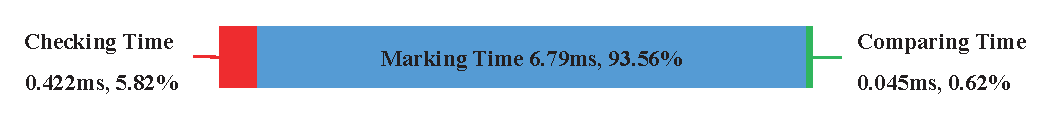
\includegraphics[width=9cm]{figures/ReinTimeDistribution.eps}
\caption{The matching time distribution of REIN}
\label{RTD}
\end{figure}

When matching event, REIN \cite{REIN} iterates through each cell that contains unmatching subscriptions, and marks each mismatch in the bitset. These repeated marking operations account for most of the matching time, as shown in Fig. \ref{RTD}. 
HEM avoids marking mismatches as much as possible by a caching mechanism. Multiple cells are allocated to one group and each group has a bitset to record whether each subscription is in the group. HEM pre-marks the subscriptions in each group as mismatches in the corresponding bitset. This optimization is called the subscription pre-mark cache (SPC) method.
In this way, HEM avoids costly traversal and marking operations, and instead uses bitwise OR operations that are more efficient for hardware. 

% As shown in the green boxes in Fig. \ref{bds}, for each attribute, there are two collections of bitsets with the same size to record subscriptions of particular cell intervals,
% Every collection has $2^{b_e}$ bitsets and is jointly responsible for the low or high value end cell list of one dimension, where $b_e$ means bit exponent. For low/high value end, every bitset records subscriptions from a suffix/prefix cell list, respectively.
\subsubsection{Subscription Pre-mark Cache (SPC) Method}

Let $g$ be the number of groups and $c$ be the number of cells at LVE or HVE. 
% The next task is to  divide the cell list into a list of mythical partitions and allocate distinct size of regions to bitsets. The relation between partitions and cells is similar to the relation between cells and the value domain. 
In particular, each group $g_i$ contains a list of continuous $i*\frac{c}{g}$ cells. Since the number of bitsets at LVE or HVE is equal to the number of groups, it is reasonable to let bitset $B_i$ record the subscriptions in group $g_i$ that contains the first/last $i*\frac{c}{g}$ cells for HVE/LVE. In this way, the coverage lengths of the bitsets constitute an arithmetic sequence with a common difference of $\frac{c}{g}$ cells. 
% For any subscription stored in a cell, it is pre-marked as a mismatch in one or more bitsets of the groups that contain the cell.
% This uniform partition division and allocation mechanism can be used in each dimension.

\begin{figure}[tbp]
\centering
\includegraphics[scale=0.37]{figures/HEM.pdf}
\caption{HEM data structure}
\label{bds}
\end{figure}

% Fig. \ref{bds} shows an example structure of HEM which builds indexes on two attributes $a_1$ and $a_2$. The value domain of each attribute is divided into sixteen cells which are assigned to four groups. Specifically, at the LVE of each attribute, group $g_1$ includes cells from $c_{13}$ to $c_{16}$, $g_2$ from $c_{9}$ to $c_{16}$, $g_3$ from $c_{5}$ to $c_{16}$ and $g_4$ from $c_{1}$ to $c_{16}$. In contrast, the way of grouping cells at the HVE starts from $c_1$. The length of the bitset associated with each group is equal to the number of subscriptions $n$. Each bitset is used to mark the subscriptions stored in the cells belonging to the corresponding group.
Fig. \ref{bds} shows an example structure of HEM which builds indexes on two attributes $a_1$ and $a_2$. The value domain of each attribute is divided into sixteen cells assigned to four groups. Specifically, at the LVE of each attribute, group $g_1$ includes cells from $c_{13}$ to $c_{16}$, $g_2$ from $c_{9}$ to $c_{16}$ and so on. In contrast, the way of grouping cells at the HVE starts from $c_1$. The length of the bitset associated with each group is equal to the number of subscriptions $n$. Each bitset is used to mark the subscriptions stored in the cells belonging to the corresponding group.

\begin{table}[tbp]
\caption{Sample subscriptions}
\centering
\begin{tabular}{|c|c|c||c|c|c||c|c|c|}
\hline
~\textbf{ID}~ & {$\mathbf{a_1}$} & \textbf{$\mathbf{a_2}$} & ~\textbf{ID}~ & \textbf{$\mathbf{a_1}$} & \textbf{$\mathbf{a_2}$} & ~\textbf{ID}~ & \textbf{$\mathbf{a_1}$} & \textbf{$\mathbf{a_2}$}   \\ \hline
$S_1$ & [0.9, 0.95] & [0.8, 0.9] & $S_2$ & [0.0, 0.3] & [0.5, 0.7] & $S_3$ & [0.63, 0.69] & [0.1, 0.2] \\ \hline 
$S_4$ & [0.38, 0.76] & - & $S_5$ &  - & [0.4, 0.57] & \multicolumn{3}{c|}{-} \\ \hline
\end{tabular}
\label{sss}
\end{table}

\subsubsection{Insertion Algorithm}

Inserting a subscription $S$ into HEM has two steps. Firstly, for each predicate in $S$, according to the attribute and low/high value, the predicate value and the subscription ID are stored as a pair in the cell that covers the value. Secondly, according to the cell grouping scheme, the subscription is marked in one or more bitsets. Algorithm \ref{ist} shows the pseudo code of insertion.

\begin{algorithm}[tbp]
%    \SetAlgoNoLine  %去掉之前的竖线
  \caption{Insertion Algorithm} 
  \label{ist}
  \KwIn{Subscription $S$} 
%   \KwOut{$numBits, endBucket, bitsID, data, bits$} 
    %$id$ = $S.id$\;
    % $numBits \leftarrow 2^{b_e}$,  $S_p \leftarrow (b + numBits - 1)/numBits$\;
    \For{each predicate $p(a_i, [l, h])$ in $S$} 
    { 
        Insert a pair $(l, S.ID)$ into the cell covering $l$ and mark $S$ in the corresponding bitsets of the groups that cover the cell at LVE\;
        Insert a pair $(h, S.ID)$ into the cell covering $h$ and mark $S$ in the corresponding bitsets of the groups that cover the cell at HVE\;
    } 
    %$numSub \leftarrow numSub+1$\;
\end{algorithm}



% \begin{table}[tbp]
% \caption{Sample Subscriptions}
% \centering
% \begin{tabular}{|c|c|c|}
% \hline
% ~ID~ & $a_1$ & $a_2$  \\ \hline
% $S_1$ & [0.9, 0.95] & [0.8, 0.9] \\ \hline 
% $S_2$ & [0.0, 0.3] & [0.5, 0.7] \\ \hline 
% $S_3$ & [0.63, 0.69] & [0.1, 0.2] \\ \hline 
% $S_4$ & [0.38, 0.76] &  - \\ \hline
% $S_5$ &  - & [0.4, 0.57] \\ \hline 
% \end{tabular}
% \label{sss}
% \end{table}
% \begin{table}[tbp]
% \caption{Sample Subscriptions}
% \centering
% \begin{tabular}{|c|c|c|c|c|c|c|}
% \hline
% ~ID~ & $a_1$ & $a_2$ & & ~ID~ & $a_1$ & $a_2$  \\ \hline
% $S_1$ & [0.9, 0.95] & [0.8, 0.9] & & $S_3$ & [0.63, 0.69] & [0.1, 0.2] \\ \hline 
% $S_2$ & [0.0, 0.3] & [0.5, 0.7] & & $S_4$ & [0.38, 0.76] &  - \\ \hline
% $S_5$ &  - & [0.4, 0.57] & & \multicolumn{3}{c|}{-} \\ \hline 
% \end{tabular}
% \label{sss}
% \end{table}

Fig. \ref{bds} also shows the state of the data structure indexing the five sample subscriptions listed in Table \ref{sss}. For example, when inserting $S_1$, for its first predicate, $\lfloor0.9*16+1\rfloor=15$ and $\lfloor0.95*16+1\rfloor=16$, so $S_1$ is mapped to cell $c_{15}$ and $c_{16}$ at the LVE and HVE of $a_1$ respectively. Predicate values are omitted for brevity. Notice that $c_{15}$ is in all the four groups at the LVE, so $S_1$ is marked in the four bitsets. At the HVE, $c_{16}$ is only contained by group $g_4$, so $S_1$ is marked in the corresponding bitset $B_4$. The second predicate of $S_1$ is processed similarly.

\subsection{Matching Procedure of HEM}
\label{ba}
HEM uses a bitset $B$ to record the matching results. Each unmarked bit represents a matching subscription.
Algorithm \ref{mth} gives the matching procedure of HEM, which can be divided into six steps. The first four steps are to process each attribute-value pair of the event. 
Step 1 performs comparisons in the cell into which the event value falls at LVE and HVE respectively and marks the unmatching subscriptions in $B$ (lines 3-4).
Step 2 selects the largest-size group that does not contain the cell into which the event value falls. Note that at LVE/HVE, when the cell ID is larger or equal than $\frac{c(g-1)}{g}$ / smaller or equal than $\frac{c}{g}$, no such group is available (line 5). 
Step 3 performs bit OR operations between $B$ and the bitset of the selected group if available at LVE and HVE respectively for each nonempty attribute in the event (line 6). 
Step 4 marks the unmatching subscriptions in $B$ that are stored in the cells not covered by the selected group (line 7). 
Step 5 does a series of bit OR operations between $B$ and the bitset of the largest-size group for each null attribute of the event (line 8). When an event does not contain an attribute, all predicates defined on the attribute are not satisfied.
Step 6 checks the unmarked bits in $B$ to obtain the matching results (line 9). 
% Details of the two processes are explained in the following example.
% 
\begin{algorithm}[tbp]
%    \SetAlgoNoLine  %去掉之前的竖线
  \caption{Matching Algorithm} 
  \label{mth}
  \KwIn{Event $E$} 
  \KwOut{Matching results $B$}
    % Define a global bitset $B$ and a bool array $dimExist$\;
    Initialize a zero bitset $B$ whose length is the number of subscriptions\;
    \For{each attribute-value pair $(a_j, v)$ in Event $E$}
    { 
        Find the cell $c_l$ at LVE and $c_h$ at HVE that the attribute value falls into\; 
        Compare $v$ with the predicate values in $c_l$ and $c_h$, and marks the IDs of subscriptions as unmatching in $B$\;
        Select the largest-size group $g_l$ and $g_h$ not covering $c_l$ and $g_h$ at LVE and HVE respectively\;
        Do bit OR operations between $B$ and the bitsets of $g_l$ and $g_h$ to obtain all unmatching subscriptions of the groups if the group is not null\;
        Mark the IDs of subscriptions as unmatching for the rest unmatching cells not covered by $g_l$ and $g_h$ in $B$ at LVE and HVE respectively\;
    }
    Do ($d-\psi_E$) times of bit OR operations between $B$ and the bitset of the largest-size group to obtain the mismatches defined on null attributes of $E$\;
    Check the unmarked bits in $B$ to output matching results.
\end{algorithm}

Let event $E=\{(e_1(a_1, 0.64), e_2(a_2, 0.32)\})$ as an example. Based on the data structure shown in Fig. \ref{bds}, the first attribute-value pair $e_1$ of $E$ falls into the cell $\lfloor0.64*16+1\rfloor=11$ on $a_1$.
The low/high values of the predicates stored in cell $c_{11}$ need to be compared with $e_1$ one by one at LVE/HVE respectively. Since the low value 0.63 of $S_3$ in $c_{11}$ is smaller than the event value 0.64, it is not marked as unmatching in $B$. 
Next, $B_1 (10000)$ and $B_2 (01000)$ are selected to do bit OR operations with $B$ since $g_1$ and $g_2$ are the largest-size group that does not cover $c_{11}$ at the LVE and HVE of $a_1$ respectively. As a result, $B = (11000)$. 
Subsequently, cell $c_{12}$ at LVE and cells $c_9$ and $c_{10}$ at HVE should be traversed since they store unmatching subscriptions and are not covered by the selected groups. In this case, there are no subscriptions to be marked as unmatching in $B$. %(Fig. \ref{ebl}). 
In REIN \cite{REIN}, cells from $c_{12}$ to $c_{16}$ at LVE and from $c_1$ to $c_{10}$ at HVE need to be traversed one by one,  %(Green line in Fig. \ref{ebcd}) 
but in HEM only three cells need to be traversed. %(Cyan line). 
The second attribute-value pair $e_2$ in $E$ is processed similarly. At the comparing step, $S_5$ stored in cell $c_7$ at the LVE of $a_2$ is marked as unmatching in $B(11001)$. $B_2 (11000)$ and $B_1 (00100)$ at the LVE and HVE respectively of $a_2$ do bit OR operations with $B$. 
At the final checking step, $B (11101)$ has one unmarked bit, meaning that $S_4$ is the match of $E$. 

HEM reduces the traversal and marking operations in the matching process by setting up a set of caches that pre-mark certain subscriptions as unmatching. Therefore, HEM mainly does bit OR operations when matching events. Generally,  compared to marking each unmatching subscription by traversing each cell, it is more efficient to perform a bit OR operation to collectively mark the unmatching subscriptions stored in multiple cells. When the selected largest-size group covers all the cells that need to be traversed, the marking time of HEM can be optimized to be close to zero. For each attribute, the total number of cells to be traversed at LVE and HVE is a constant, namely $\frac{c}{g}-1$.



\section{Theoretical Analysis}
\label{ta}

\subsection{Complexity Analysis}
% In this section, we analyze the time and space complexity of three algorithms introduced in section \ref{ba}. 
% Other three optimizations differ in initialization, insertion and matching process but they would not cause much more time and space, so their complexity analysis is omitted.

% It is easy to see that the time complexity of Initialization Algorithm is $O(d)$. The size of $endBucket$ and $bitsID$ array is $O(d)$. The size of $data$ array is $O(d*b)$ because no subscription is inserted at this time. A bitset needs a space of $n$ bits. So the size of $bits$ array is $O(n*d*g)$. In total, the space complexity of Initialization Algorithm is $O(d*(b+n*g))$.

\paragraph{Time Complexity of Insertion Algorithm.} For a subscription $S$ with size $\psi_S$,  it needs to insert $2\psi_S$ pairs into the corresponding cells, which takes $O(\psi_S)$. In addition, marking the subscription in one or more bitsets has a cost at most $O(g\psi_S)$. Therefore, the time complexity of insertion is $O(g\psi_S)$.
% The additional space overhead is $O(1)$.
% The loop in line 2 takes $O(\psi_S)$ to process each predicate of the subscription. 

\paragraph{Time Complexity of Matching Algorithm.} The matching procedure of HEM can be divided into six steps to analyze. 
The comparison step (Lines 3-4) checks pairs in two cells with average cost $O(\frac{n\psi_S}{dc})$. 
The cost of two bit OR operations (Lines 5-6) is $O(n)$.
The marking step (Line 7) traverses $\frac{c}{g}-1$ cells for both value ends, so the cost is $O(\frac{n\psi_S}{dc}*(\frac{c}{g}-1))=O(\frac{n\psi_S}{dg})$. Given the event size $\psi_E$, these three steps have a cost $O(\psi_En(1+\frac{\psi_S}{dg}))$ since $g\le c$. The time to process null attributes (Line 8) is $O((d-\psi_E)n)$. The final check step (Line 9) takes $O(n)$. Therefore, the time complexity of the matching algorithm is $O(dn+\frac{n\psi_E\psi_S}{dg})$. 
% If the bit OR operation is seen as the basic unit, the time complexity of HEM is $O(d+\frac{n\psi_E\psi_S}{dg})$. 

\paragraph{Space Complexity.} Given the dimensionality $d$ of the content space and the number of cells $c$ divided on each attribute, the total number of cells is $dc$. The total number of bitsets is $2dg$. For $n$ subscriptions with size $\psi_S$, the total number of predicates is $n\psi_S$. Thus, the space complexity of HEM is $O(dc+dng+n\psi_S)$.

\subsection{Performance Analysis}
\label{peim}
In this section, we build a analysis model for HEM to quantify the relationship between performance improvement and memory consumption. To explore the improvement on marking time, we take the HVE of one attribute as a breakthrough since the LVE and HVE of each attribute have similar characteristics.

\begin{lemma}
\label{lemma1}
Given the number of subscriptions $n$ with size $\psi_S$, the marking time of HEM is proportional to $0.5n\psi_S$ without the SPC method.
\end{lemma}
\begin{proof}
The marking time of HEM is proportional to the times of marking subscriptions one by one, which is computed as:
    \begin{equation}
        n\psi_S\int_0^1(x-0)dx=0.5n\psi_S
    \end{equation}
where $dx$ can be seen as a probability and x is the possible value of an event. The interval range to be traversed is $[0,x]$. \qed
\end{proof}

\begin{lemma}
\label{lemma2}
Given $n,\psi_S$ and $g$, the marking time of HEM is halved by doubling $g$ with the SPC method. %the marking time is proportional to $\frac{n}{2^{b_e+1}}$.
\end{lemma}
\begin{proof}
The adoption of the SPC method limits the number of traversing cells to $\frac{c}{g}-1$. Hence, with the SPC method, the number of marked subscriptions is computed as:
    \begin{equation}
\begin{aligned}
    \label{eq1}
        & n\psi_S\sum_{i=0}^{g-1}\int_\frac{i}{g}^{\frac{i+1}{g}}(x-\frac{i}{g})dx  \\ 
        = {} & n\psi_S\int_0^1xdx-\frac{n}{g}\psi_S\sum_{i=0}^{g-1} i\int_\frac{i}{g}^{\frac{i+1}{g}}1dx \\
        = {} & 0.5n\psi_S-\frac{(g-1)n\psi_S}{2g} = \frac{n\psi_S}{2g} 
    \end{aligned}
    \end{equation}
where $x-\frac{i}{g}$ is the length of interval to be marked one by one for any event value $x\in [\frac{i}{g}, \frac{i+1}{g}], i\in[0,g-1]$. Since the marking time is proportional to the times of marking subscriptions one by one, doubling $g$ halves the marking time. \qed
\end{proof}


\begin{theorem}
\label{theorem1}
Given $n,\psi_E,\psi_S, d$ and $g$, when $\psi_E=d,g>1$ and the predicate values are uniformly distributed in the value domain $[0,1]$, the improvement ratio of the marking time of HEM is $1-\frac{1}{g}$ with the SPC method.
\end{theorem}
\begin{proof}
Based on Lemma \ref{lemma1} and \ref{lemma2}, the improvement ratio of the marking tasks of HEM is $1 - \frac{n\psi_S}{2g*0.5n\psi_S} =1-\frac{1}{g}$. \qed
\end{proof}
% 结论1、2

Theorem 1 means that 50\% or 96.875\% of marking operations are avoided when $g$ is set to 2 or 32 respectively, presenting an inverse proportional relationship. The ratio does not hold when $g=1$ because it assumes that the unique bitset on LVE or HVE covers all cells. Nevertheless, we can configure that the unique bitset on LVE or HVE covers only half of the cells when $g=1$. Thus, the improvement of $g=1$ is equivalent to that of $g=2$ when $\psi_E=d$. 

\label{qip}

% \begin{corollary}
% Let $\frac{\psi_E}{d}=q\textless1$, the improvement proportion on marking time is $1-\frac{q}{g}$.
% \end{corollary}

% \begin{proof}
% If events have not definitions on $d-\psi_E$ dimensions, the marking tasks on these dimensions are all replaced by bit OR operations. According to Lemma \ref{lemma2}, the marking time will be about $\frac{q*n}{2^{b_e+1}}$ and the improvement proportion will be about $1-\frac{q*n}{2^{b_e+1}*0.5n}=1-\frac{q}{g}$. QED. 
% \end{proof}

% 结论3、4
% Suppose $q$ is 0.5 and $b_e$ is 3,the marking workload can be reduced by 93.75\%.

% 结论567
% As is discussed in section \ref{sdrop}, the space complexity increases exponentially with $b_e$, but we can apply the double reverse optimization to lessen the marking load by $93.75\%$ with $b_e=3$ and $q=1$ or $b_e=2$ and $q=0.5$. The memory to store bitsets decreases by half. 

% \label{pi}

% % 结论8
% In reality, absolute uniform distribution of predicate values is impossible. In this situation, the dynamic partition optimization evaluates the marking task load in a more rational and dynamic criterion, making the actual improvement proportion on marking time closer to the theoretical value. 


% % 结论9
% The state reduction optimization devotes to lessening the bit or operation time under the high-dimensional space. A group whose size is $g$ can reduce the bit or operation time to $\frac{1}{g}$ of the original.


% \subsection{Bottleneck Analysis}
% The matching time of HEM consists of five components: comparison time, marking time, bit or operation time, count time. Each component can be a bottleneck under certain circumstance. In this section, we give the factors for each component to become a bottleneck.

% \textbf{Comparison Time ($T_{cmp}$):} When $c$ is small, $n$, $\psi_S$, $\psi_E$, $b_e$ is big and event values always fall into cells close to the far left/right end of partitions at high/low value end, the comparing workload will be large relatively and only a few cells should be traversed for marking subscriptions, now the $T_{cmp}$ becomes a bottleneck.

% \textbf{Marking Time ($T_m$):} When $b_e$ is small, $c$ is big, event values and predicate values are uniformly distributed, the $T_m$ is a bottleneck. This is the most common scenario. In addition, increasing $n, \psi_S$ or $\psi_E$ may also poses a increase of $T_m$.

% \textbf{Bit OR Operation Time ($T_O$):} For each event of size $\psi_E$, the number of bit OR operations is up to $2*\psi_E+(d-\psi_E)=d+\psi_E$. Typically, increasing $\psi_E$ will increase the marking time more quickly than the increase of $T_O$. Thus, when $d$ is very large, the $T_O$ becomes a bottleneck. Meanwhile, if $n$, $\psi_S$ is small and $b_e$ is big, the amount of comparing and marking will decline. Consequently, the ratio of $T_O$ is relatively large.


% \textbf{Count Time ($T_{cnt}$):} 
% When the other three types of time are all quite small, the $T_{cnt}$ will be a bottleneck. The number of bits to be checked is $n$. A high matching probability causes a big number of additions on the number of matching subscriptions. Therefore, the condition is: small $d, \psi_S, \psi_E$, big $n, w, b_e$. 


% \section{Achievement}
% \label{ac}
%  This section illustrates how to implement $HEMDD$ and $HEMSR$ from the points of data structure. Different from Fig. \ref{bds}, we use two arrays to store the (predicate value, subscription ID) pairs and collections of bitsets separately. One is $data$ and the other is $bits$. Besides, there are four auxiliary arrays to record state information: $endBucket, bitsID, doubleReverse, fix$. 
 
%  For all arrays, the first layer is to index low and high value ends while the second layer is to index dimensions. For $data$ array, the third layer is to index cells and the fourth layer is to index pairs in the cell. 
 
%  The third layer of $bits$ array is to index bitsets. The last bitset in both value ends is identical, so we use an extra two-dimensional array named $fullBits$ to store all the subscription IDs in each dimension. The fourth layer  of $bits$ and the second layer of $fullBits$ is to index the subscription IDs. The true value in subscript i of the last layer means the subscription whose ID is i is in the bitset. For $HEMSR$, there is an additional array termed $bitsSR$ to store the bitsets calculated by bit or operations of $g$ bitsets in a group, which can be seen as the result of bit or operations in $g$ dimensions. The first layer of $bitsSR$ is to index groups and the second layer indexes the combined bitsets. For instance, suppose $g$ is 5, the binary of 22 is $10110_2$, so $bitsSR[1][22]$ means the bitset derived by bitsets at LVEs of sixth and ninth dimension and bitsets at high value ends of seventh, eighth and tenth dimension.
 
% $endBucket$, $bitsID$, $doubleReverse$ and $fix$ arrays all have three dimensions and index cells in the third layer. $endBucket$ array records the farthest cell number to be traversed. When the marking direction is from low cell to high cell, the number should plus one for convenience. $bitsID$ array stores the ID of bitset that can be exploited by the matching process of current event. When the value of $bitsID$ is $2^{b_e}-1$, it is time to use the bitset in $fullBits$ other than $bits$ array. $doubleReverse$ is a bool array, recording whether to use the double reverse optimization for each cell event values fall into. $fix$ array is used in calculating task load (the number of pairs) for dynamic partition and dynamic double reverse optimization. At HVE, it records the prefix sum of the number of pairs in cells while at LVE it records the suffix sum. We take $fix[0][1][0]=500,000$, $fix[0][1][3]=490,000$, and $fix[0][1][12]=375,000$ as an example. The dynamic partitions are drawn in Fig. \ref{dpm}. Suppose an event value falls into cell 2 in dimension 1. The marking task load by double reverse optimization (bucket 0 to 2) is 10,000 pairs while the load by single reverse method (bucket 3 to 11) is 115,000 pairs. Since 10,000 is smaller than 115,000, it is better to use the bitset with wider coverage, namely, $fullBits[1]$. Therefore, $endBucket[0][1][2]=0$, $bitsID[0][1][2]=3$, $doubleReverse[0][1][2]=true$.
 
% Finally, there are two special circumstances that should be treated specifically. Firstly, when $b_e=0$, there is only one bitset in charge of half of workloads in low or high value end of one dimension and $fullBits$ array is omitted. Half of workloads should be traversed in all null dimensions of events. Secondly, in static partition method, when the number of partitions can not divide the number of cells, the sizes of the first $2^{b_e}-1$ partitions are the same and bigger than the size of the last partition. However, the partition number starts from the high cell end at the LVE. Thus, the last partition at LVE is a strict subset of the first partition at HVE. For consistency, we make the HVE share its partition set with the LVE, so the last partition at LVE is identical to the first partition at HVE. 

\section{Experiments}
\label{ex}

\subsection{Setup}

\subsubsection{Workloads}
% 暂时没有默认值,这一节包括表都需要修改
% We synthesize subscriptions and events workloads based on BEGen \cite{Be-tree}.
The event data comes from a real-world stock dataset with 50 attributes after being cleaned up. The dataset was collected from the Chinese stock market on June 8, 2018. The subscription data is generated based on the stock dataset. For high-dimensional testing, we synthesize event data.
Table \ref{psd} lists the parameter settings where the default values are marked in bold. 
% The performance of event matching algorithms is affected by many parameters. We change their settings to observe their effects as listed in Table \ref{psd} where $M$ represents one million. The default value of each parameter is marked in bold. 
% The Zipf distribution with parameter $ \alpha$\cite{zipf} is used to simulate the skewness of attributes and predicate values. 

% In order to avoid matching zero subscription, we generate the proportion $p$ of subscriptions and events that are defined on the first $\psi_S$ and $\psi_E$ attributes separately. 
% under circumstance with diverse event types
% The last four parameters can be randomly selected from a value range to comprehensively test algorithms in a dynamic environment. 
% and Normal Distribution
% \vspace{-0.4cm}

\begin{table}[tbp]
\caption{Parameter settings in the experiments}
\centering
\label{psd}
\begin{tabular}{|c|l|l|}
\hline
Name & Description & Experimental Values  \\ \hline
% $p$ & Subscription or event proportion defined & 0, \textbf{0.5} \\
%     &  on the first  $\psi_S$  or  $\psi_E$ attributes. & \\ \hline 
 $\mathcal{R}$ & The value domain of attribute. & $[1,1M]$ \\ \hline
 $\alpha$ & Parameter of Zipf. &  \textbf{0}, 1 $\sim$ 5 \\ \hline %0, 0.5, 1, 1.5, 2
$d$      & Number of attributes. &  \textbf{20}, 30, 100, 300 $\sim$ 900   \\ \hline
$n$      & Number of subscriptions. & 0.3M, \textbf{1M}, 3M $\sim$ 9M \\ \hline
$\psi_E$      & Event Size.  & \textbf{20}, 30 $\sim$ 80 \\ \hline
$\psi_S$      & Subscription size. & 5, \textbf{10}, 15 $\sim$ 30      \\ \hline
$w$ & Predicate width. & 0.1, 0.2, \textbf{0.3} $\sim$ 0.9 \\ \hline
% $c$  & Number of cells. & 30, 100, 500, \textbf{1k}, 1.5k, 2k \\ \hline
% $b_e$ & Bit exponent. & 0, 1, 2, 3, 4, 5, 6, 7, 8  \\ \hline
% $g$ & Dimensional group size. & 2 $\sim$ 10 \\ \hline
\end{tabular}
\end{table}



\subsubsection{Baselines}
We compare HEM with four event matching algorithms reviewed in Section \ref{rw}, namely REIN \cite{REIN}, Ada-REIN \cite{Ada-REIN}, TAMA \cite{TAMA} and OpIndex \cite{OpIndex}. Based on REIN, Ada-REIN ignores some marking tasks on attributes to reduce matching time, resulting in some false positive matches. REIN and Ada-REIN originally only support single-type event matching ($\psi_E=d$). We re-implemented them to match events with multiple types, namely $\psi_E \ll d$. Besides, they are set with the same $c$ as HEM (1,000 by default). The false positive rate of Ada-REIN is set to 0.05. TAMA counts the matching predicates for each subscription which exist only in $\psi_E$ attributes. The discretization level of TAMA is set to 13. We re-implemented TAMA to achieve exact matching with negligible overhead. OpIndex classifies subscriptions by their pivot attributes and only pivot attributes of events are processed.  

% In addition, we design two brute force algorithms as baselines: $Simple$ and $Simple2$. $Simple$ compares the predicates of each subscription with event values one by one. It will stop matching once a unmatching predicate is encountered and continue to judge the next subscription. $Simple2$ is the same as $Simple$ except sorting the predicates based on width before inserting a subscription. When $w$ is fixed, $Simple$ is the baseline; otherwise, $Simple2$ is the baseline.
%In MO-Tree, the number of levels is set to 4, the height of tree is set to 6, the threshold on the number of cells stabbed by a value is set to 6.5 and the number of disjoint cells is set to 10.
% 10 for more obvious acceleration effect than REIN. 
\subsubsection{Testbed}
All the algorithms are implemented in C++ language and compiled by g++ 9.3.0 with -O3 optimization enabled on Ubuntu 20.04 system. All the experiments are conducted on an AMD 3.7 GHz machine with 64 GB RAM.
% All algorithms are encapsulated in an executable file and a core is appointed to run all algorithms alone at once. 
% The amount of codes for implementing HEM and its variants is about four thousands non-blank and non-comment lines. 
% Extra log information is removed in formal experiments.


\subsubsection{Metrics}
We evaluate the performance of the five algorithms in terms of three metrics: matching time, insertion time and memory consumption. The matching time is measured from the beginning of matching an event to the end of obtaining the whole matching result. 500 events are processed to calculate the average matching time in each experiment. 
% For brevity, the average number of matching subscriptions of 500 events is designated as an answer to verify the correctness. 
Insertion time refers to the time of inserting a subscription into the data structure. 
Memory consumption refers to the total memory used by the underlying data structure of the matching algorithm after inserting a subscription dataset.
% We also investigate the four components of matching time in HEM.
% a deletion task of randomly selected 5 k subscriptions
%  constructing time, 
%  Constructing time is the initialization time for the data structure with a input subscriptions set. 
% the matching function returns the number of matching subscriptions as the matching result.
% constructing and 
\subsection{Verification Experiments}
We design a benchmark experiment to verify the performance analysis model in Section \ref{peim} and investigate the trade-off between matching time and memory usage. In this experiment, the parameters are set to the default values.
% investigate the change of matching time composition with $g$.  

% 证明了5.2节的结论1、2、3
Fig. \ref{mthb} presents the marking time of HEM with different number of groups $g$ from 1 to 512. Starting from $g=2$, the marking time of HEM halves for each time $g$ is doubled. For example, the marking time is 0.60 ms and 0.31 ms for $g=16$ and $g=32$ respectively. 
In this experiment, we set $\psi_E=d$, so the group covering all the cells is not used. Consequently, the marking time for $g=1$ is approximately equal to that for $g=2$. The average marking time without the SPC method is 6.79 ms, smaller than twice of the marking time when $g=2$. This is because the groups are statically divided and the predicates are not absolutely evenly distributed. 
When $g=32$, the performance improvement ratio of HEM is $1 - \frac{0.31}{6.79}\approx95.4\%$, which is close to the theoretical value 96.875\% based on Theorem \ref{theorem1}. 
% The predicate width 0.3 poses some unused bitsets.
Overall, the ratio of marking time in the total matching time decreases from 93.7\% to 2.5\% when $g$ increases from 1 to 512, indicating that the bottleneck operation (Fig. \ref{RTD}) has been alleviated. In summary, the SPC optimization method is effective and Theorem \ref{theorem1} is validated. 

% components of matching time.
% verify their efficacy
% of six HEM versions in Table \ref{sbm} 
% Experimental parameters are: $d=20, \psi_S=10, \psi_E=20, n=1m, w=0.3$. 
% The average number of matching subscriptions is 6.558 for every method.
% This suggests that all the algorithms are implemented correctly in matching logic.

% \subsubsection{HEMPS Experiment}

\begin{figure}[tbp]
\centering
\begin{minipage}[t]{0.48\textwidth}
\centering
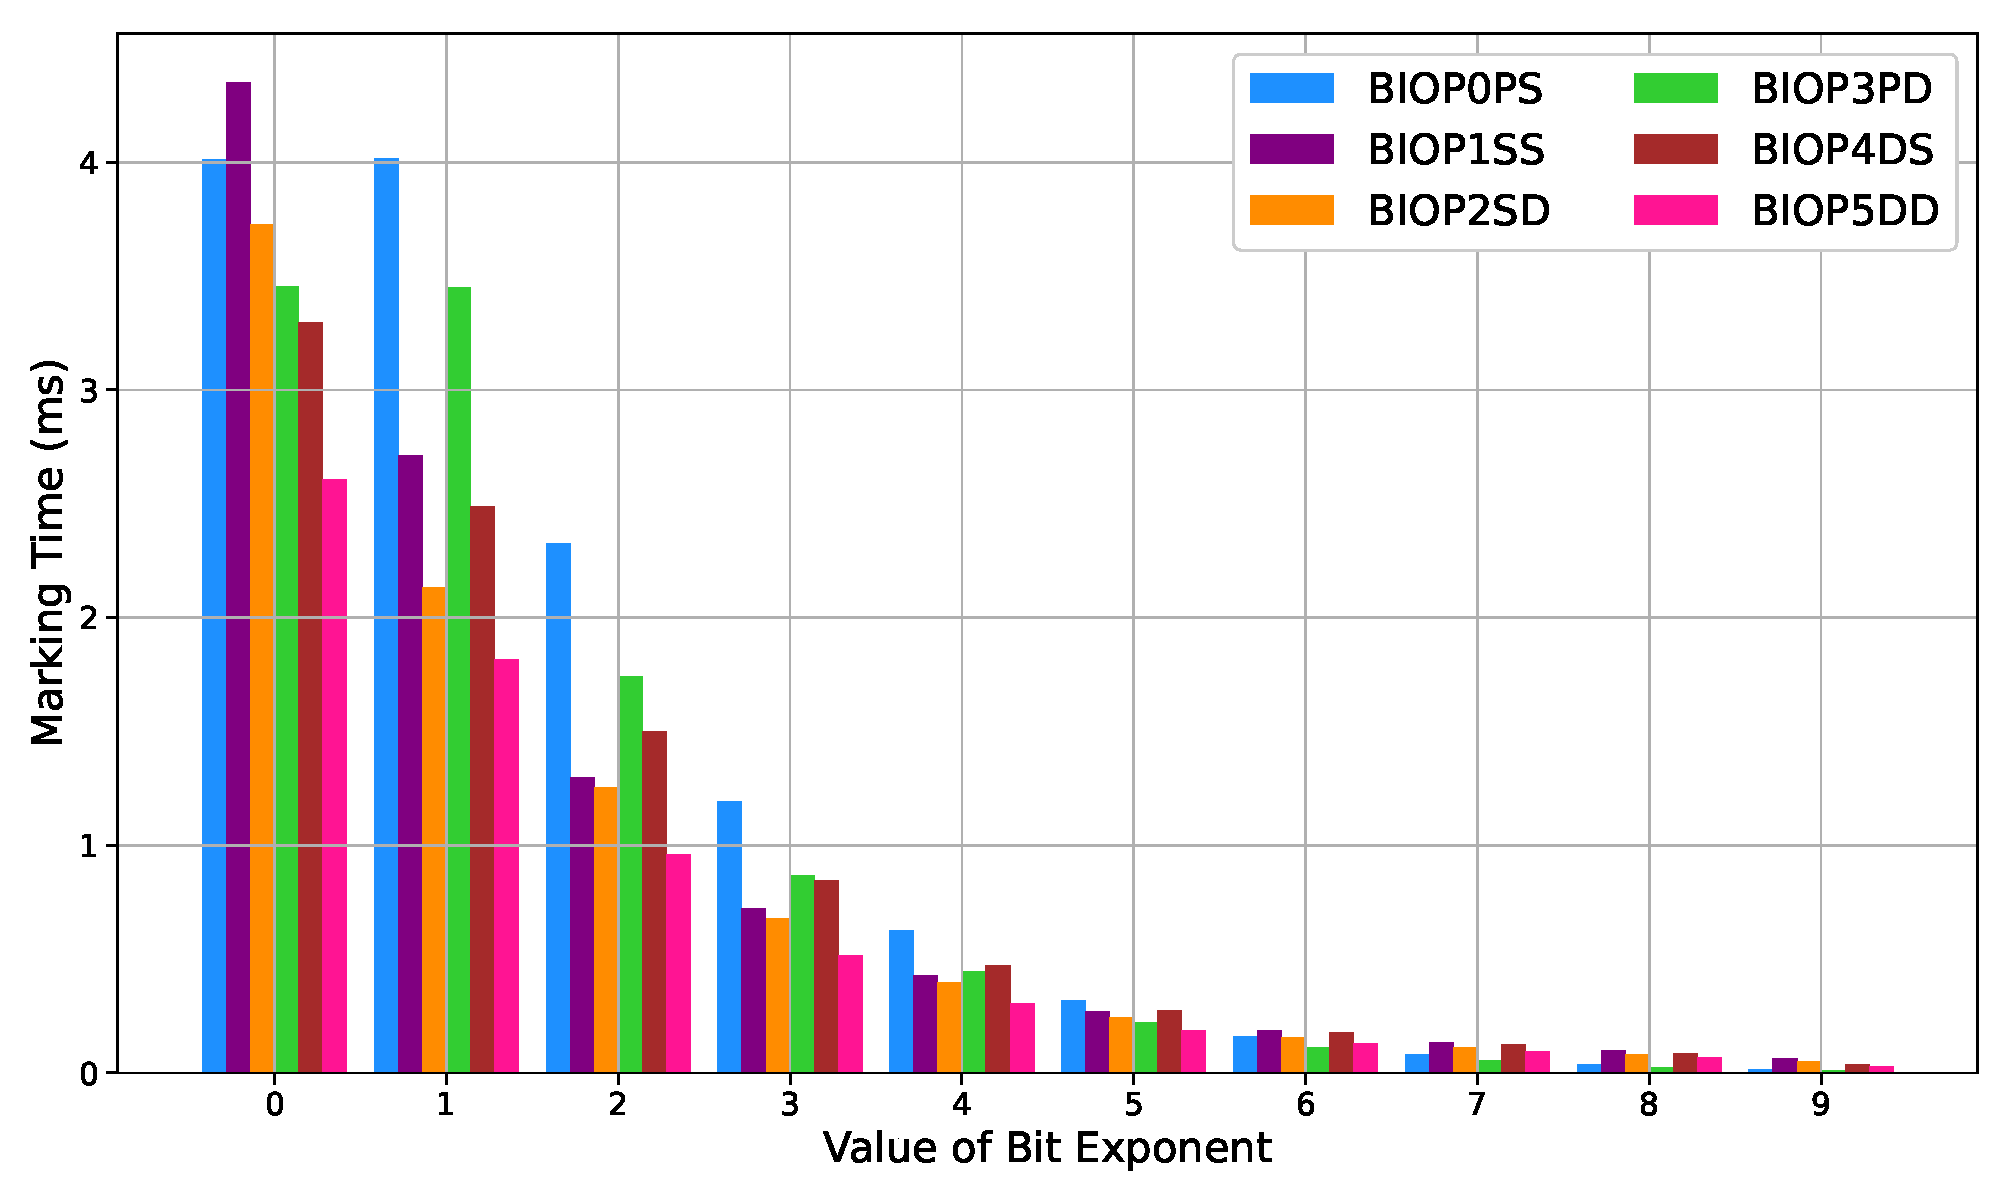
\includegraphics[width=4.8cm]{figures/bemarking.eps}
% \vspace{-0.3cm}
\caption{Marking time of HEM with different $g$}
\label{mthb}
\end{minipage}
\quad
\begin{minipage}[t]{0.48\textwidth}
\centering
 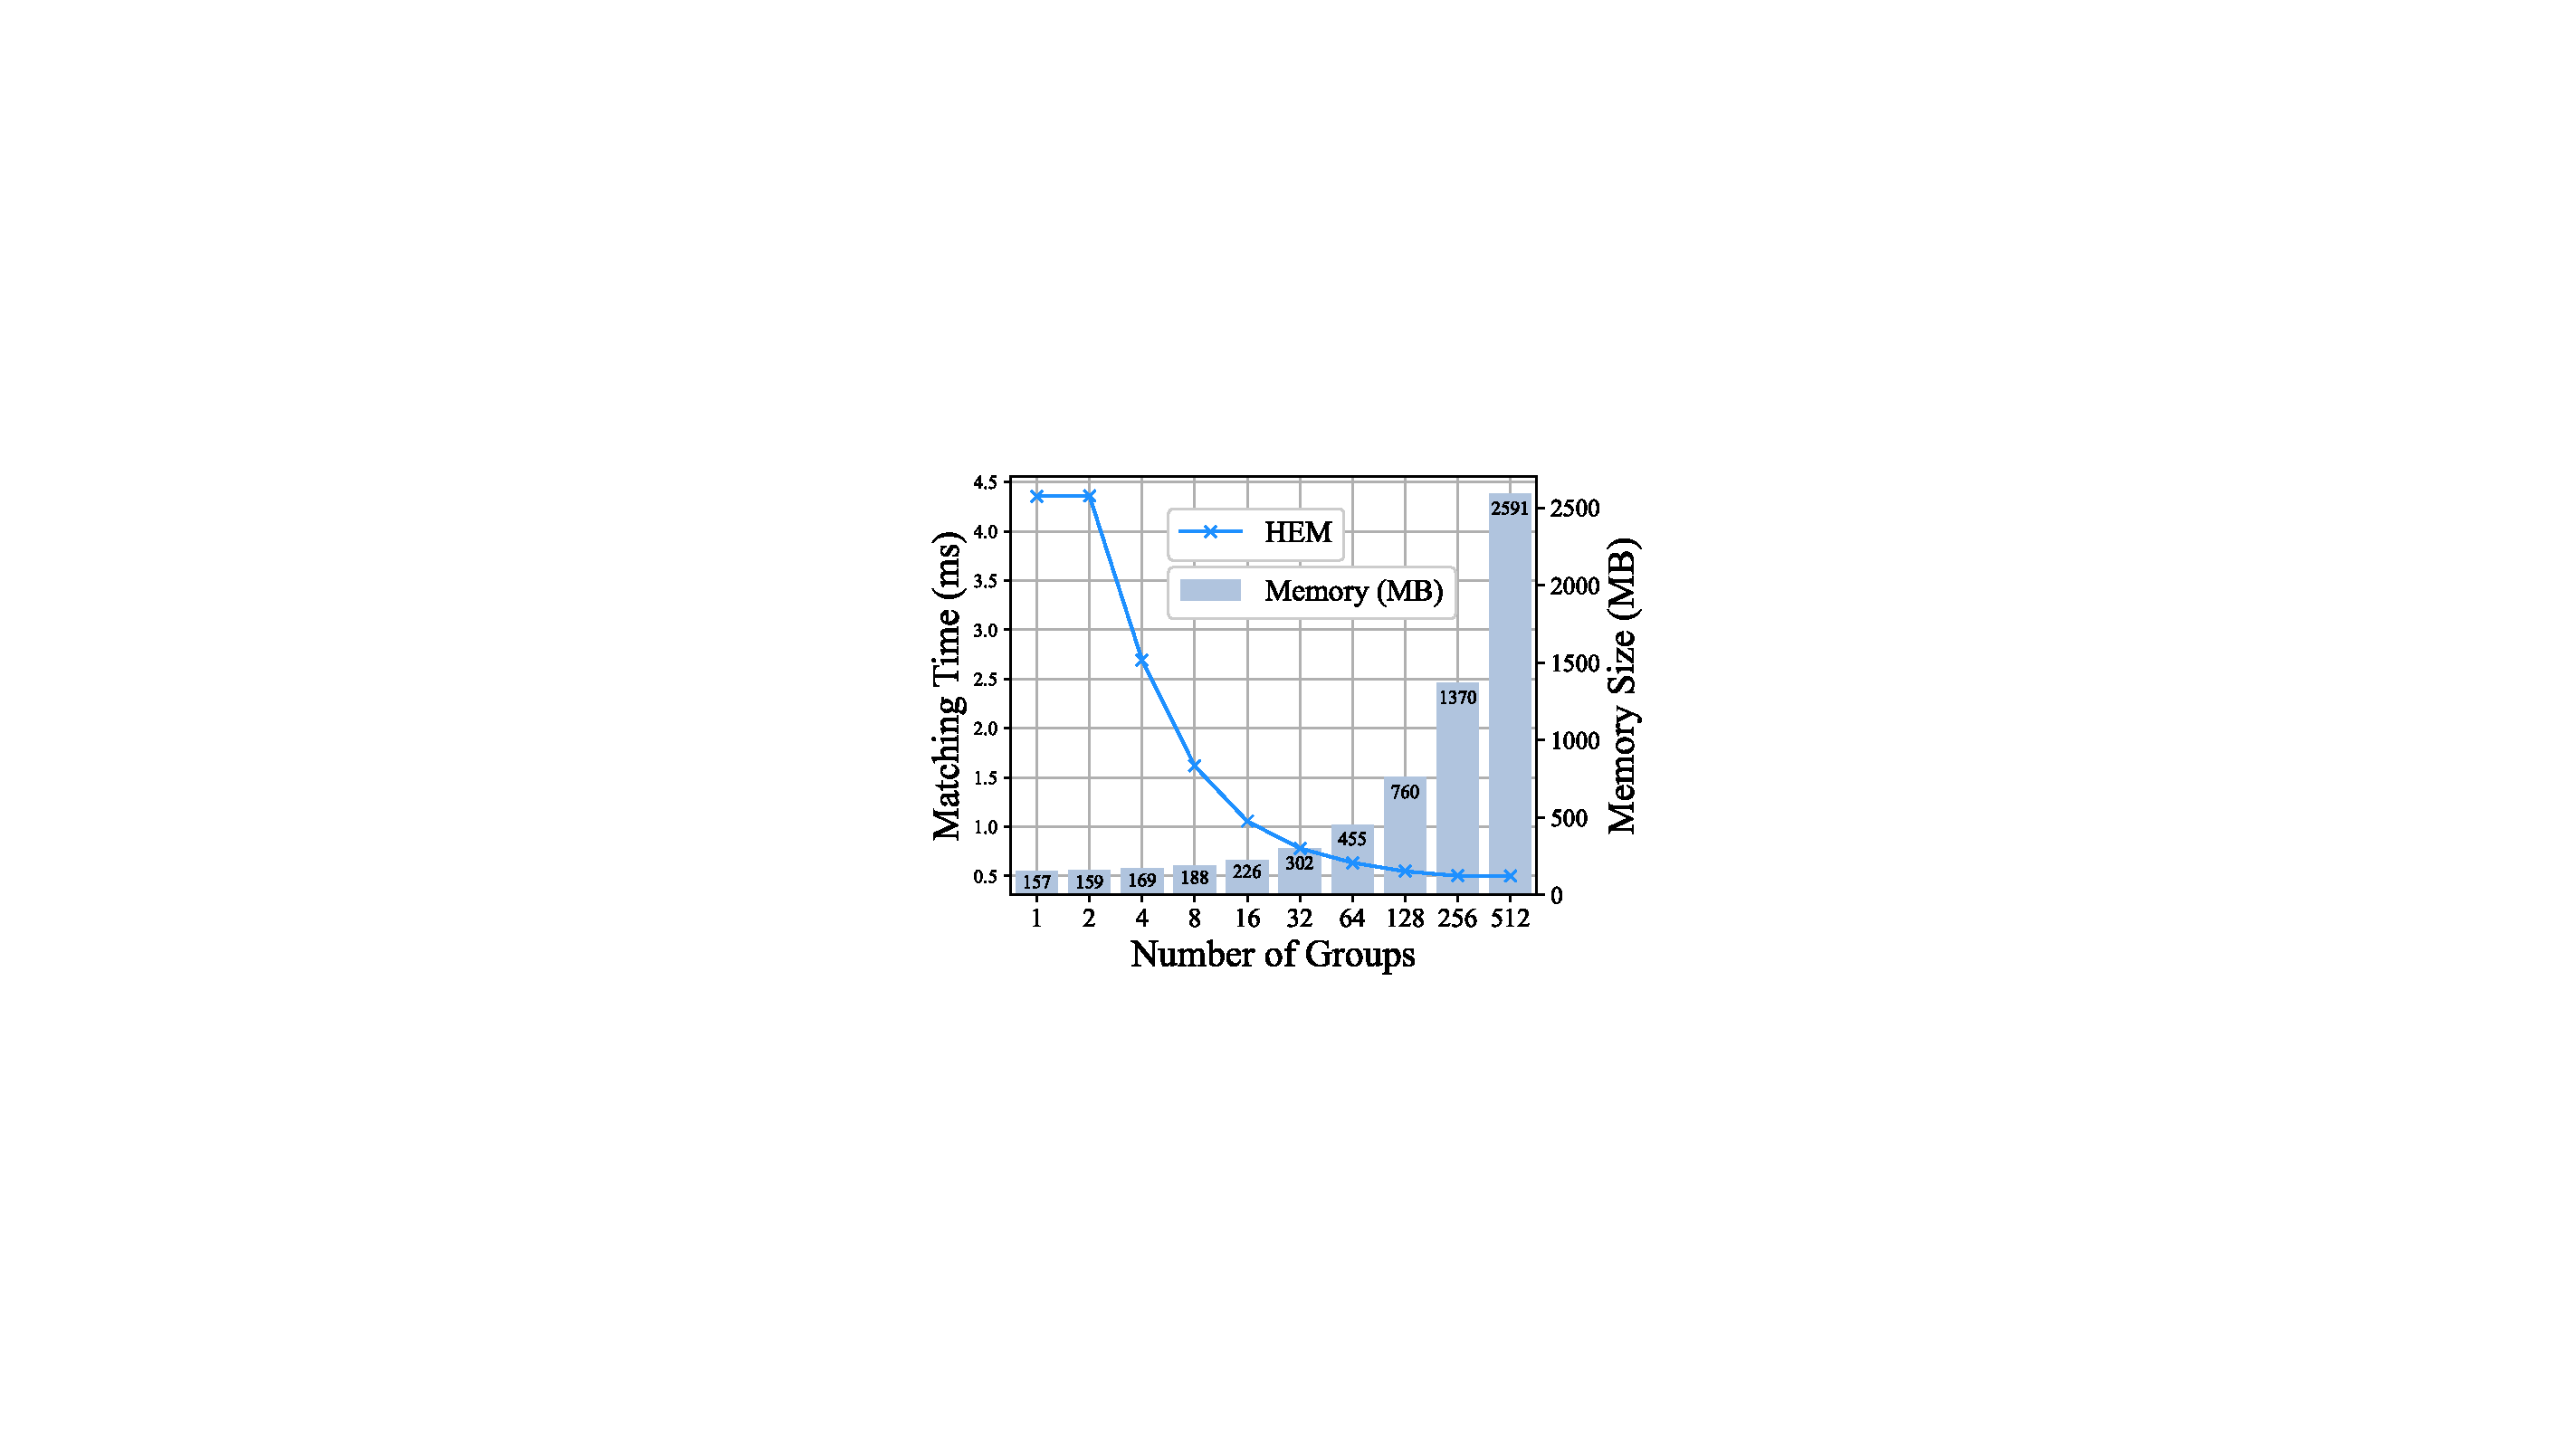
\includegraphics[width=5.7cm]{figures/matchingTime.eps}
\caption{Matching time and memory usage of HEM with different $g$}
\label{mtmc}
\end{minipage}
\end{figure}



% 证明了5.2节的结论5
% $HEM1SS$ performs better than $HEM0PS$ when $b_e$ is 1 to 5. For example, the marking time of $HEM1SS$ when $b_e$ equals to 2 is 1.297 ms, slightly larger than 1.194 ms, the marking time of $HEM0PS$ when $b_e$ is 3. This means the static double reverse optimization works. However, it does not work when $b_e$ is 0. This is because the width $w$ is 0.3, and partition 0 in Fig. \ref{dro} has no predicates. When an event value falls into cell 10, it is dispensable to traverse cell 11 to 19, which contain many predicates. The number of cells is not appropriate to be the indicator of marking workload in this situation. In addition, when $b_e$ is bigger than 5, there is less room for optimization of marking tasks. The double reverse optimization deals with the marking task of low and HVE separately, posing a lower cache hit rate. These two points cause $HEM1SS$ being inferior to $HEM0PS$ and $HEM4DS$ being inferior to $HEM3PD$ when $b_e$ is big. Distinct to $HEM0PS$, the marking time of $HEM1SS$ with $b_e = 1$ is less than that with $b_e=0$, indicating that the bitsets covering all the partitions are utilized for double reverse matching. Besides, the improvement proportion of $HEM1SS$ is $1-\frac{0.722}{6.827}\approx89.42\%$ when $b_e$ is 3, slightly less than 90.6\%. In conclusion, the double reverse optimization is feasible and the related deduction in section \ref{pi} is verified.

% % 证明了5.2节的结论8
% Overall, the dynamic partition variants ($HEM3PD$, $HEM2SD$, HEM) are always superior to their corresponding static variants ($HEM0PS$, $HEM1SS$, $HEM4DS$) and their improvement proportions are closer to the theoretical values. When $b_e$ is 3, the improvement proportion of HEM is $1-\frac{0.515}{6.827}\approx 92.46\%$. Due to the same reason as the double reverse optimization, $HEM0PS$ outweighs $HEM2SD$ and $HEM3PD$ outweighs HEM when $b_e$ is bigger than 6 and 5, respectively. Thus, $HEM3PD$ has the highest improvement proportion 99.8\% on marking time when $b_e$ is 9.

% \begin{figure}[htbp]
% \centering
% \begin{minipage}[t]{0.48\textwidth}
% \centering
% \includegraphics[width=6cm]{figures/BIOP5DDTimeDistributionByBe.eps}
% \caption{Exp1: Time Distribution of HEM5DD by $b_e$}
% \label{biop5ddtd}
% \end{minipage}
% \quad
% \begin{minipage}[t]{0.48\textwidth}
% \centering
%  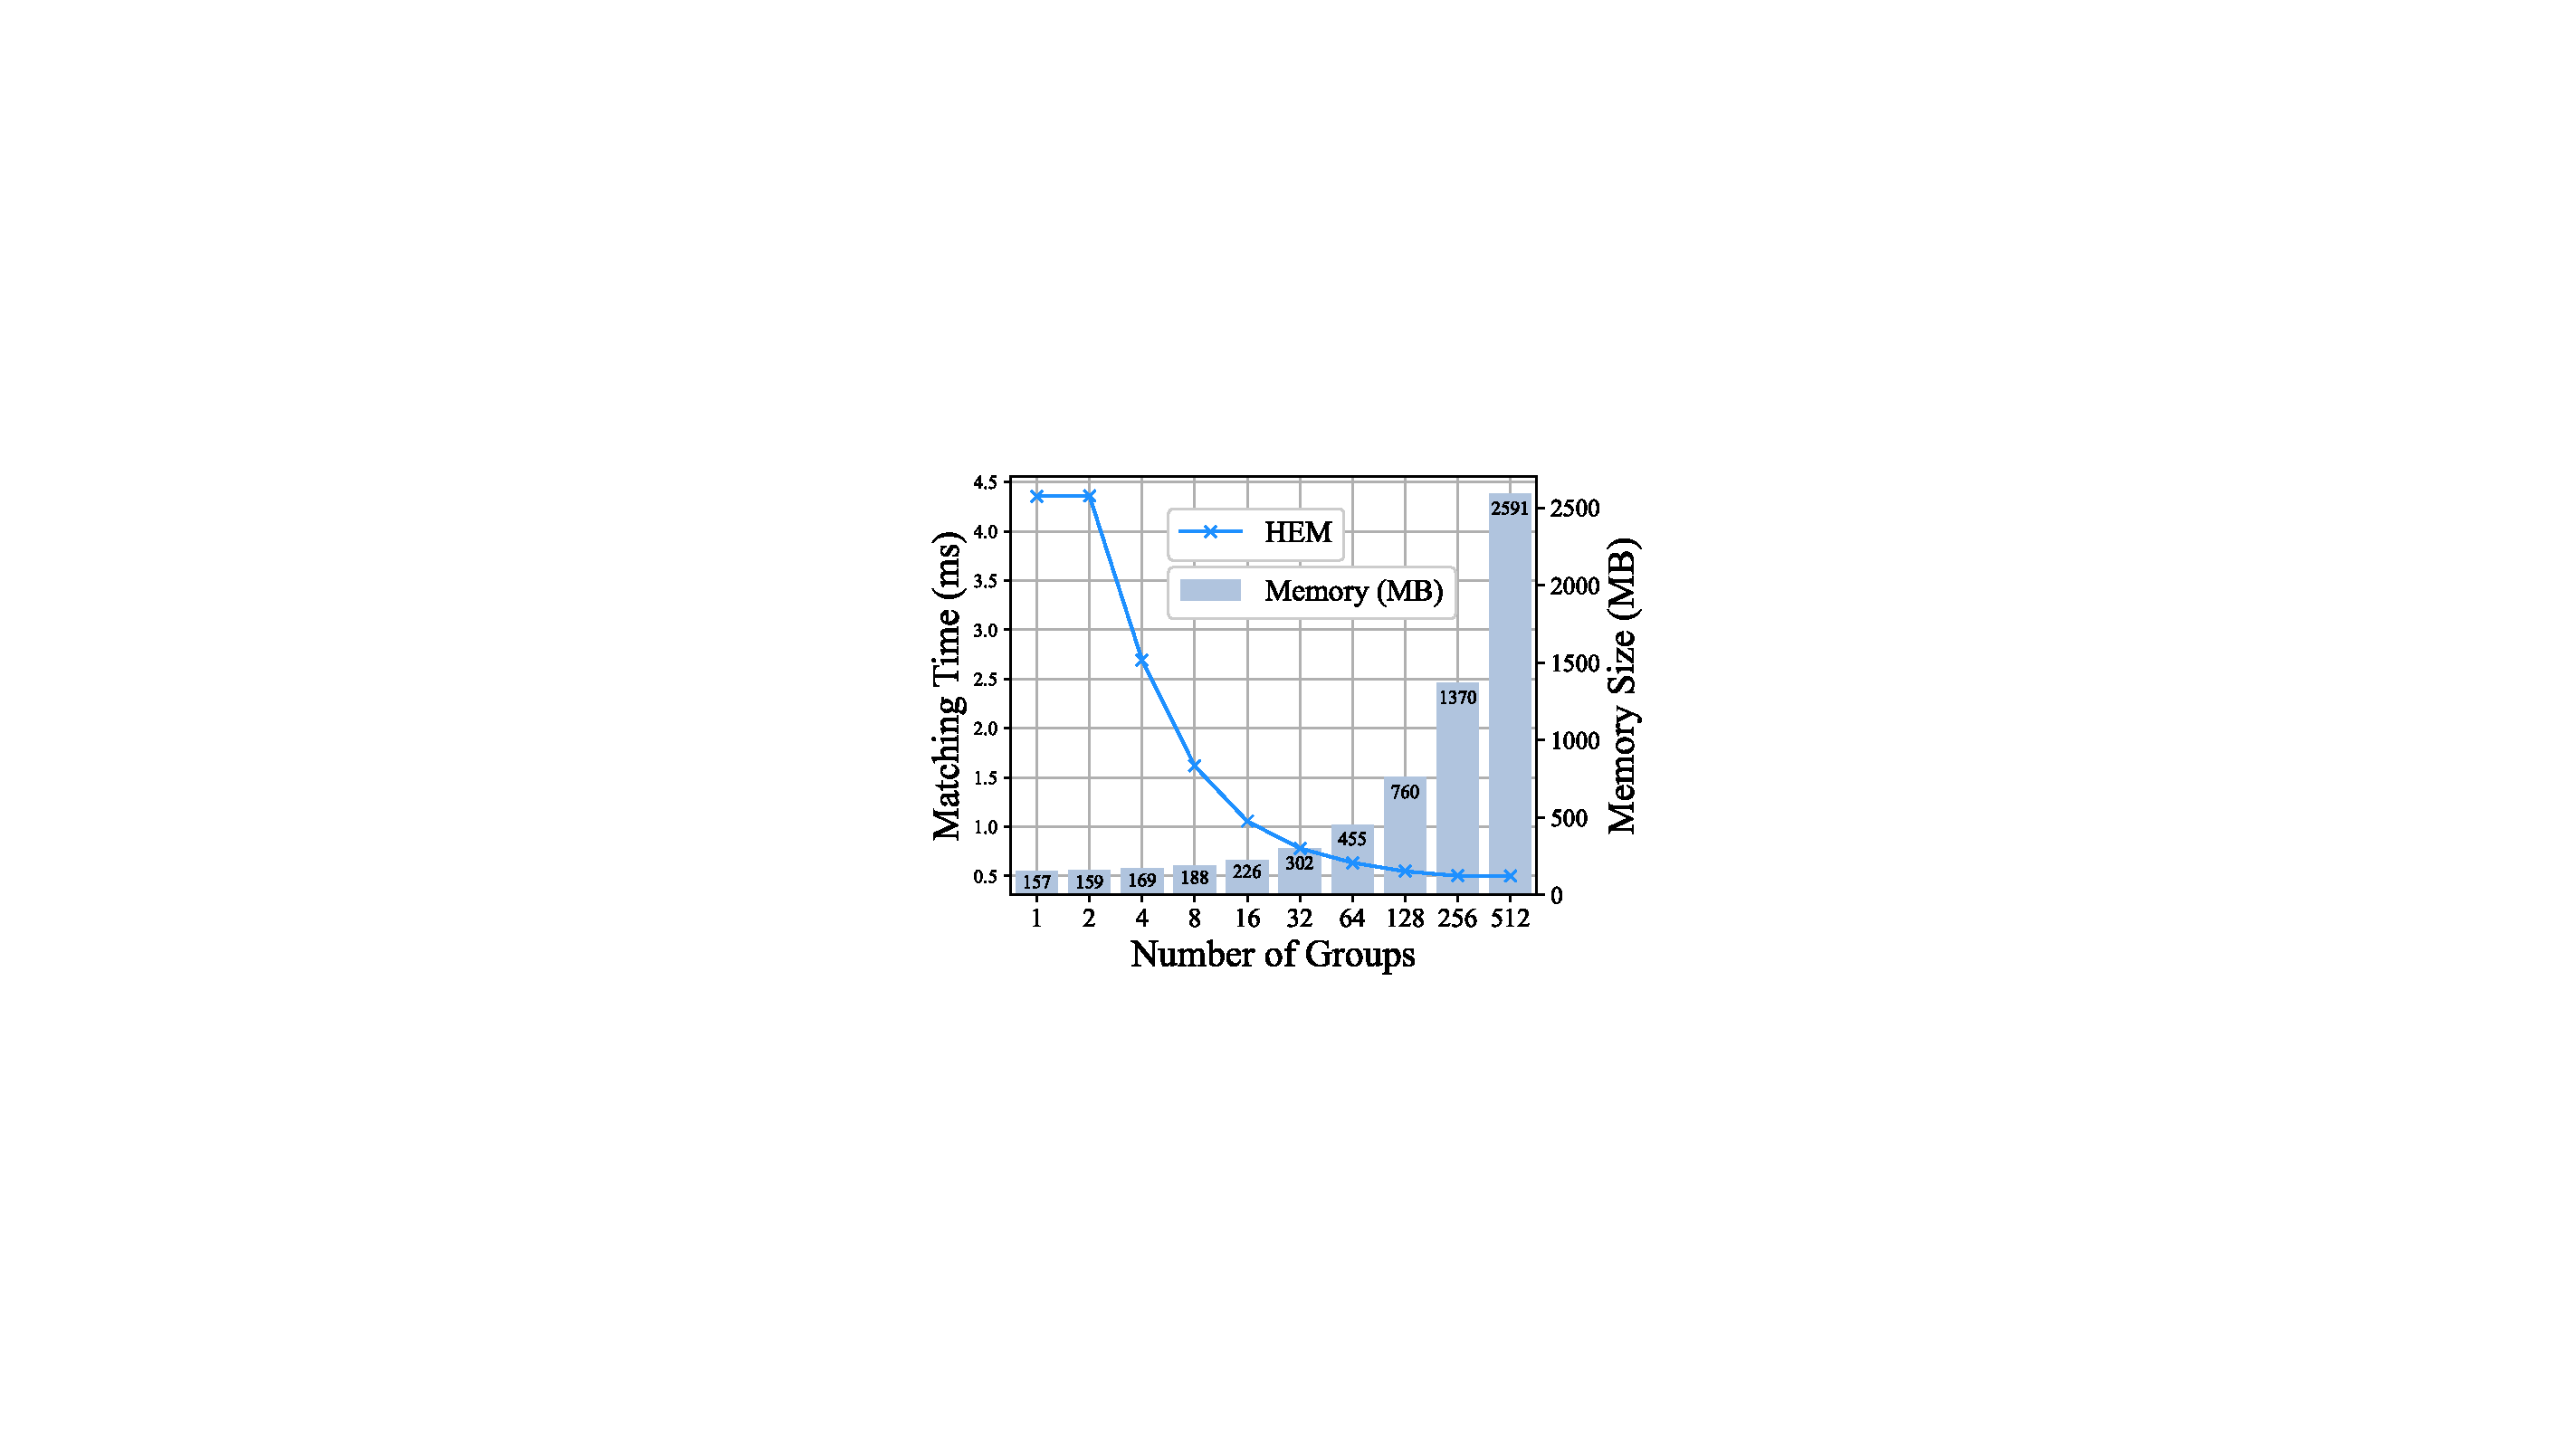
\includegraphics[width=6cm]{figures/matchingTime.eps}
% \caption{Exp1: Matching Time and Memory of HEM and HEM5DD by $b_e$}
% \label{mtm1}
% \end{minipage}
% \end{figure}

% \begin{figure}[htbp]
% \centering
% \includegraphics[width=7cm]{figures/HEM5DDTimeDistributionByBe.eps}
% \caption{Exp1: Time Distribution of HEM5DD by $b_e$}
% \label{biop5ddtd}
% \end{figure}

% \begin{figure}[htbp]
% \centering
% 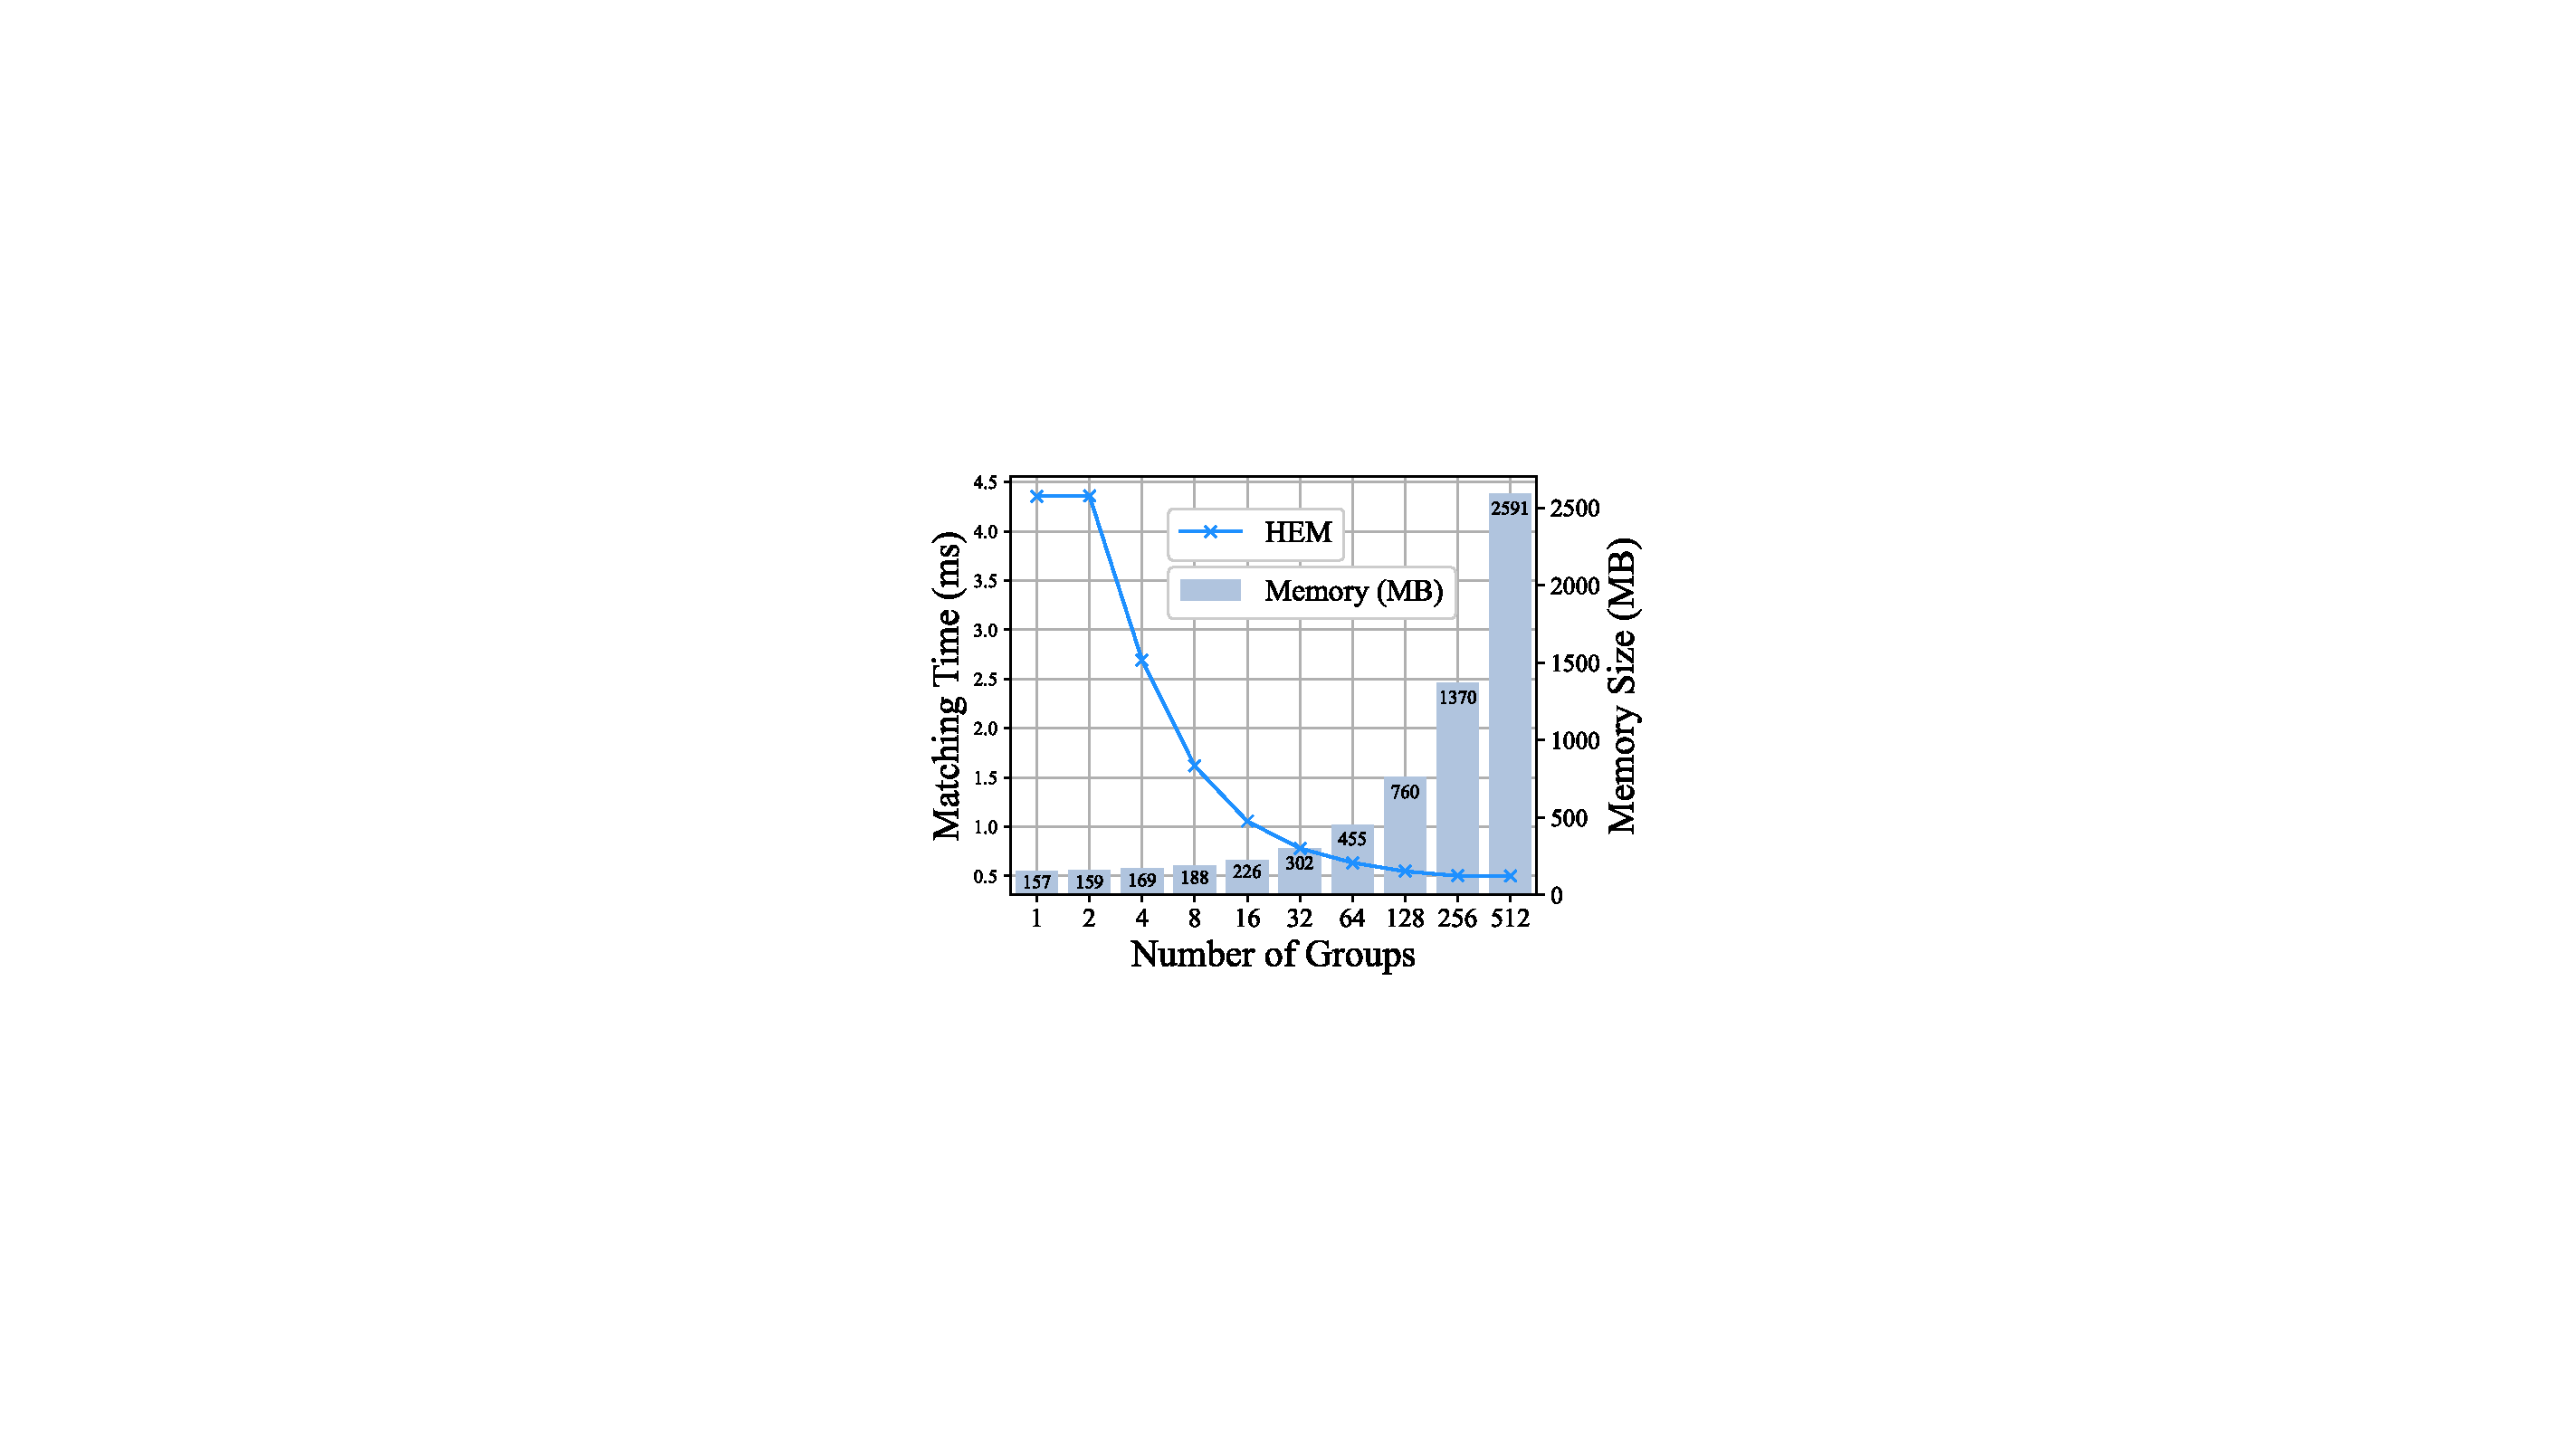
\includegraphics[width=8cm]{figures/matchingTime.eps}
% \caption{Exp1: Matching Time and Memory of HEM and HEM5DD by $b_e$}
% \label{mtm1}
% \end{figure}

Fig. \ref{mtmc} depicts the matching time and memory usage of HEM varying $g$ from 1 to 512. The matching time dwindles exponentially and the memory usage grows exponentially with the exponential increase of $g$. When the SPC optimization method is not enabled, the matching time of HEM is 7.56 ms and the memory consumption is 152 MB. We finally set $g=32$ to do the metric experiments since the matching time of HEM drops by 89.7\% and the memory usage is nearly doubled, which makes a good trade-off.

% Fig. \ref{hemtd} shows how $g$ affects the time distribution of HEM. The proportion of marking time decreases from 93.7\% to 2.5\%. With the increase of $g$, the workload of comparison and counting is immutable and the workload of bit OR operations increases. Their shares keep rising with $b_e$ relatively due to the relative decline of marking time. The bottleneck (Marking Time) has been alleviated. When $g$ is 32, the proportion of bit OR time and marking time is relatively uniform. Therefore, we set $g$ to 32 in the metric experiments.
% 这段结尾有点突兀,但与下一段的结尾对应



% 证明了5.2节的结论7
% Fig. \ref{mtm1} shows the matching time and memory size of $HEM0PS$ and HEM. The difference of $HEM0PS$ and HEM is less than 1 MB so the memory of HEM is omitted. Without the help of bitset collections, the average matching time is 7.5 ms and the memory size is 152 MB. The added memory mainly concentrates on bitset collections. The size of bitsets is $2*n*d*2^{b_e}\approx 4.768*2^{b_e} MB$. For example, when $b_e$ is 3, the memory size is $152+4.768*2^3\approx 190.1$ MB. $38.1$ MB is added. Nevertheless, we design the $fullBits$ (see Section \ref{ac}) array to avoid storing the complete subscription IDs twice in each attribute. Therefore, the memory size is $190.1 MB - 1 mb *20*1\approx 187.7 MB$, which is consistent with the experimental result. Increasing $b_e$ by one, the theoretical memory size will be $152+38.1*2- 0.12*20\approx 225.8 MB$ . Thus, decreasing $b_e$ by one, the memory to store bitsets decreases by half. From Fig. \ref{mtm1} we can see that the matching time of $HEM0PS$ with $b_e = x$ is less than the matching time of HEM with $b_e = x+1$ where $x=0 \sim 3$. This is due to the joint contribution of double reverse optimization and dynamic partition optimization. The matching time is reduced by up to 89.9\% when $b_e$ is 9. Combined with Fig. \ref{biop5ddtd} and \ref{mtm1}, we choose HEM version and $b_e=4$ to do the metric experiments in next section.

% \begin{figure}[htbp]
% \centering
% \includegraphics[width=5cm]{figures/exp2_marking_Se.eps}
% \caption{Exp2: Marking Time when $\frac{\psi_E}{d}=q=0.5$ and $p=0.5$}
% \label{exp2ms}
% \end{figure}

% 证明了5.2节的结论4、6
% Fig. \ref{exp2ms} illustrates that the improvement proportion $1-\frac{q}{g}$ in section \ref{qip} is correct where $q=\frac{\psi_E}{d}$. $HEM3PD\_20\psi_E$ is same as $HEM3PD$ in Experiment 1. In Experiment 2, we set $\psi_E=10, p=0.5$ so that $q=0.5$ and the average number of matching subscriptions is not zero. The marking time of $HEM3PD\_10\psi_E$ and $HEM5DD\_10\psi_E$ is 0.502 ms and 0.527 ms when $b_e$ is 3 and 2, respectively,  so the improvement proportion is $\frac{0.502}{6.827}\approx 92.65\%$ and $\frac{0.527}{6.827}\approx 92.28\%$, similar to that of $HEM3PD\_20\psi_E$ with a marking time 0.445 ms when $b_e$ is 4. The difference is caused by the parameter $p$. If we set $p=0$, the marking time of $HEM3PD\_10\psi_E$ and $HEM5DD\_10\psi_E$ can be 0.424 ms and 0.471 ms when $b_e$ is 3 and 2, separately.

\subsection{Metric Experiments}
The performance of the event matching algorithm is affected by many parameters. We change their settings to observe their effects in the experiments.
% Based on real stock data set, we evaluate the matching time of five matching algorithms by control variable method. In each metric experiment, the default values in Table \ref{psd} are adopted if no otherwise specified. %$p$ is set to 0 in Experiment 5 and 7.

% \begin{figure}[htbp]
%     \centering
% 	\subfigbottomskip=2pt %两行子图之间的行间距
% 	\subfigcapskip=-5pt %设置子图与子标题之间的距离
%     \subfigure[Exp3: Varying $n$]{
%         \centering
%         \includegraphics[width=3.7cm]{figures/exp3_n.eps}
%         \label{exp3}
%     }
%     \quad
%     \subfigure[Exp4: Varying $\psi_S$]{
%         \centering
%         \includegraphics[width=3.7cm]{figures/exp4_Ss.eps}
%         \label{exp4}
%     }
%      \subfigure[Exp5: Varying $\psi_E$]{
%         \centering
%         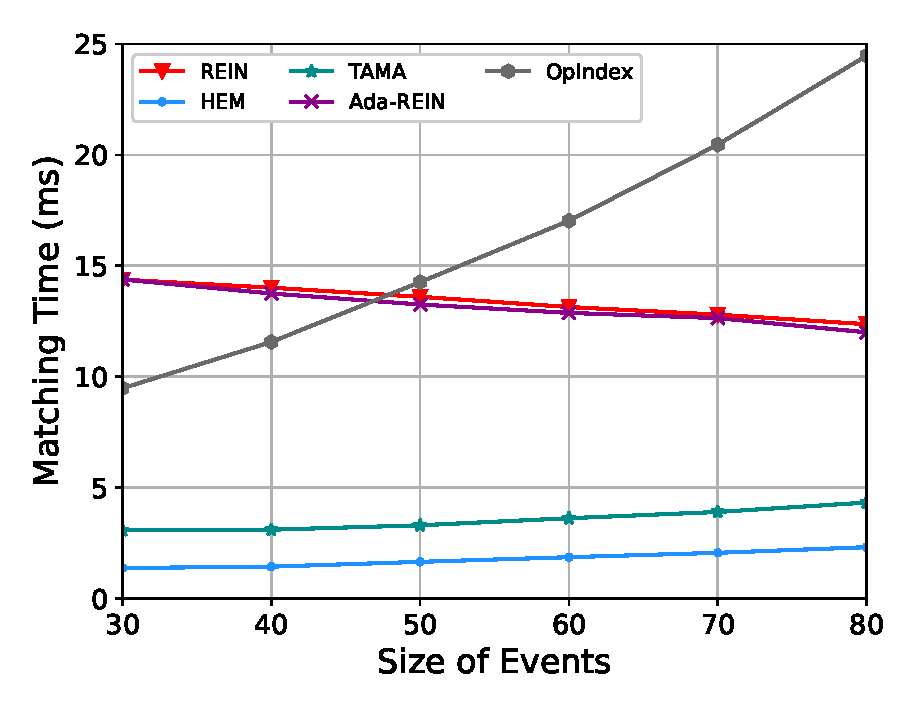
\includegraphics[width=3.7cm]{figures/exp5_Se.eps}
%         \label{exp5}
%     }
%     \quad
%     \subfigure[Exp6: Varying $w$]{
%         \centering
%         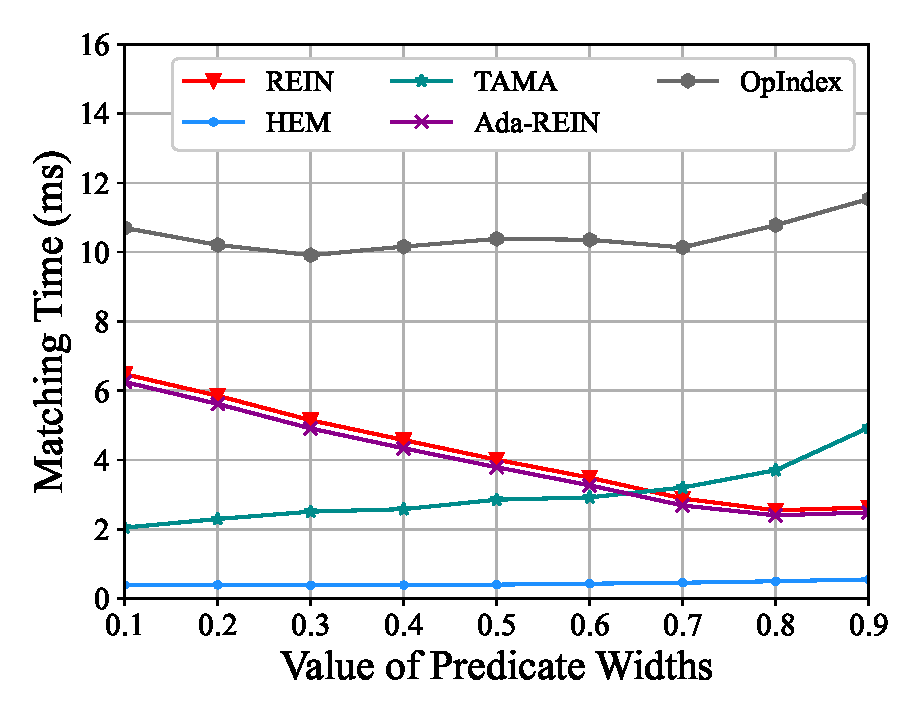
\includegraphics[width=3.7cm]{figures/exp6_w.eps}
%         \label{exp6}
%     }
%      \subfigure[Exp7: Varying $d$]{
%         \centering
%         \includegraphics[width=3.7cm]{figures/exp7_d.eps}
%         \label{exp7}
%     }
%     \quad
%     \subfigure[Exp8: Varying $\alpha$ of Zipf Distribution]{
%         \centering
%         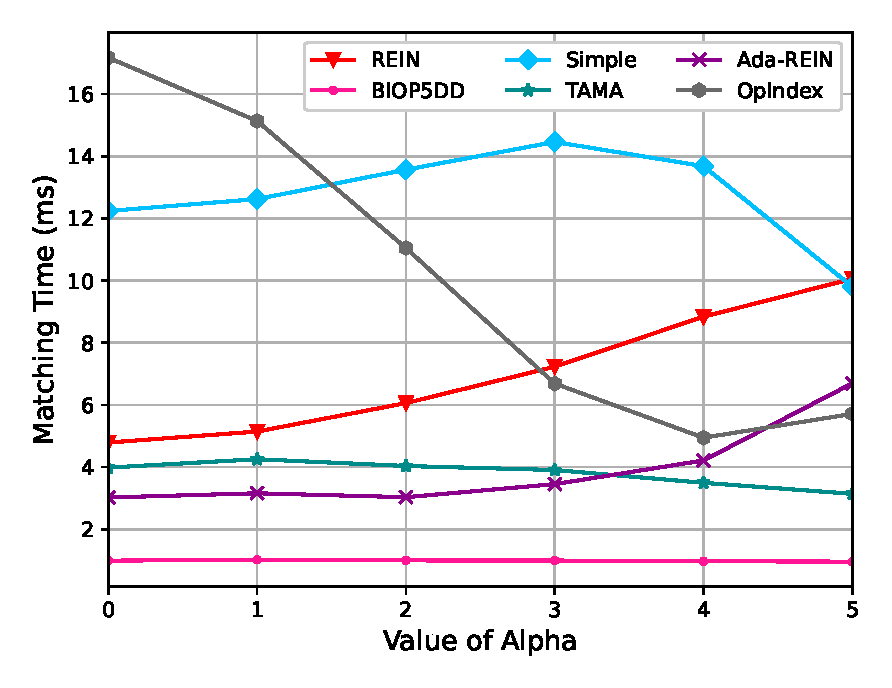
\includegraphics[width=3.7cm]{figures/exp8_alpha.eps}
%         \label{exp8}
%     }
% \caption{Matching Time of Six Metric Experiments}
% \end{figure}

\subsubsection{Number of Subscriptions $n$.}
The number of subscriptions is a core parameter to measure the workload, which has a vital impact on the matching time. As shown in Fig. \ref{exp3}, all algorithms have higher matching time as $n$ increases. HEM performs best in all situations. Compared with REIN, TAMA, Ada-REIN and OpIndex, HEM reduces the matching time by 90.1\%, 83.5\%, 90.0\% and 95.9\% respectively on average. When $n$ grows from 3M to 7M, the predicates become more densely distributed in the cells and the optimization space becomes larger. Hence, the matching time of HEM increases slower than before. When $n$ is 9M, the matching time of HEM grows more quickly because the bit OR operations cost a lot. The matching time of TAMA increases faster than REIN and Ada-REIN because the workload of counting satisfied predicates is time-consuming. OpIndex performs worst because predicates are evenly distributed in attributes and all the attributes are elected as pivot attributes.

\begin{figure}[tbp]
\centering
\begin{minipage}[t]{0.48\textwidth}
\centering
\includegraphics[width=5cm]{figures/exp3_n.eps}
\caption{Effect of $n$}
\label{exp3}
\end{minipage}
\begin{minipage}[t]{0.48\textwidth}
\centering
 \includegraphics[width=5cm]{figures/exp4_Ss.eps}
\caption{Effect of $\psi_S$}
\label{exp4}
\end{minipage}
\end{figure}
% 

\subsubsection{Subscription Size $\psi_S$.}
To measure the effect of $\psi_S$, we set $d=\psi_E=30, w=0.7$ and vary $\psi_S$ from 5 to 30. From Fig. \ref{exp4} we can see that the matching time of the five algorithms increases linearly with $\psi_S$. Therefore, $\psi_S$ is more related to the real workload compared to $n$. The performance of Ada-REIN is almost the same as REIN. This is attributable to the low false positive rate, low matching probability and the uniform distribution of predicates. Compared with REIN, TAMA, Ada-REIN and OpIndex, HEM reduces the matching time by 83.7\%, 82.6\%, 83.1\% and 95.2\% respectively average.
% only the matching time of HEM does not increase with $\psi_S$. This is because the workload for marking accounts little while the counting time accounts a lot and decreases since the number of matching subscriptions is about 163 k and 30 k when $\psi_S$ is 5 and 10 separately.
% The false positive rate of Ada-REIN is 10 and the matching probability is about 0.163 when $\psi_S$ is 5, so it skips all the attributes and directly does the counting task to calculate the number of matching subscriptions. Therefore, the matching time of Ada-REIN 0.427 ms is approximately equal to the time of doing plus one operations for a million times. 

\subsubsection{Event Size $\psi_E$.}
In the event size experiment, we set $d=80$ and vary $\psi_E$ from 30 to 80. Generally, the event size is proportional to the matching time of the forward matching algorithms (TAMA and OpIndex) and inversely proportional to the matching time of the backward matching algorithms (REIN and Ada-REIN), as shown in Fig. \ref{exp5}. Nevertheless, HEM, as a backward matching algorithm, has a slowly increasing matching time with $\psi_E$. This is because both comparing and marking operations are avoided and only one bit OR operation is needed to process each null attribute. On average, the matching time of HEM is reduced by 88.5\%, 86.5\%, 86.3\% and 50.3\% compared with OpIndex, REIN, Ada-REIN and TAMA, respectively.

\begin{figure}[htbp]
\centering
\begin{minipage}[t]{0.48\textwidth}
\centering
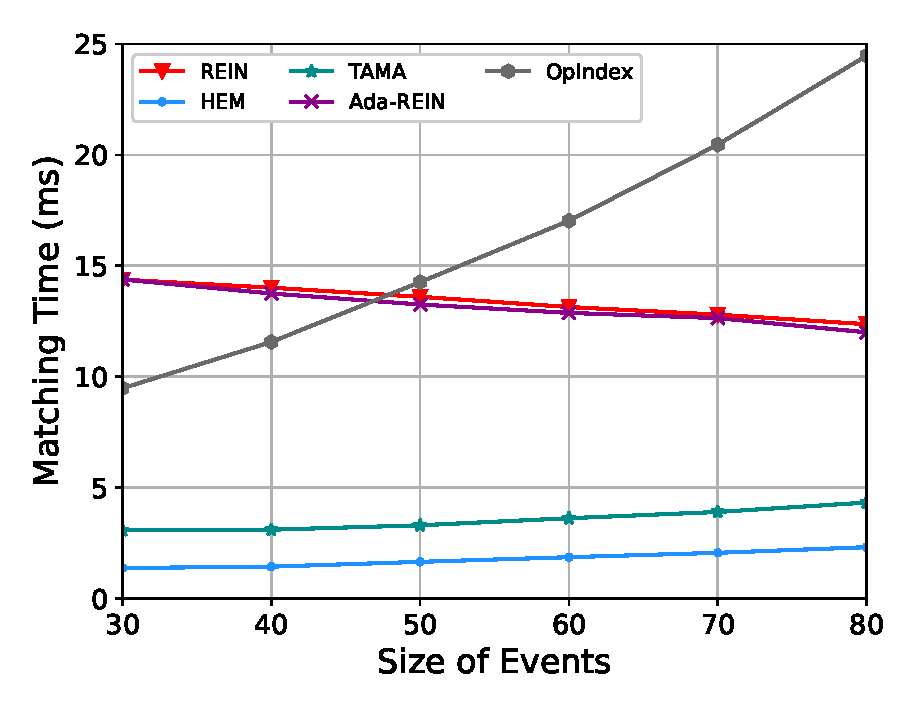
\includegraphics[width=5cm]{figures/exp5_Se.eps}
\caption{Effect of $\psi_E$}
\label{exp5}
\end{minipage}
\begin{minipage}[t]{0.48\textwidth}
\centering
 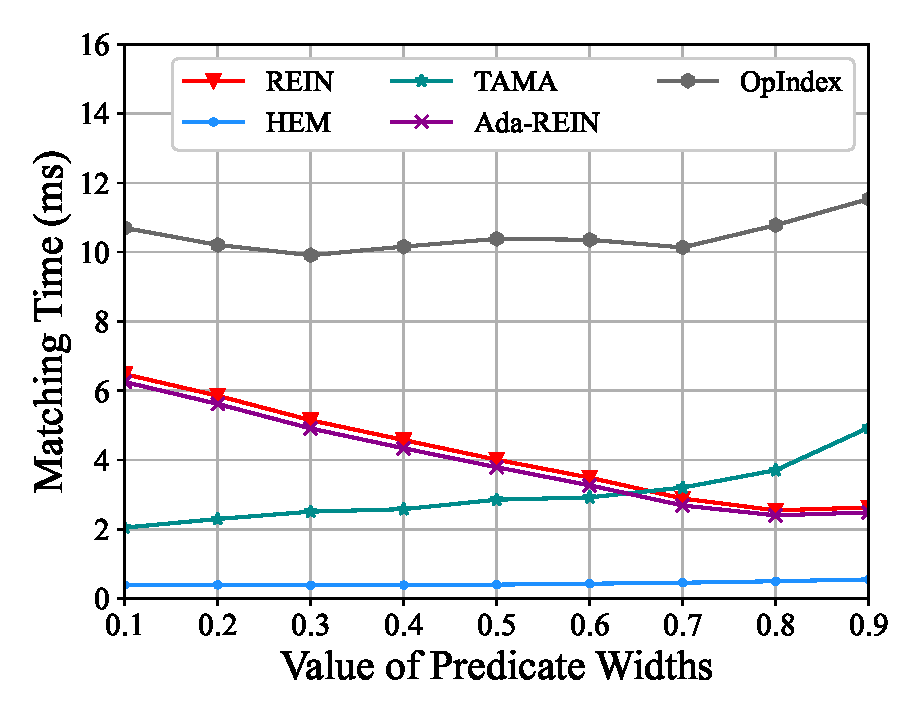
\includegraphics[width=5cm]{figures/exp6_w.eps}
\caption{Effect of $w$}
\label{exp6}
\end{minipage}
\end{figure}


\subsubsection{Predicate Width $w$.}
The matching probability of subscriptions is relevant to $\psi_S$ and $w$. Fig. \ref{exp6} presents how $w$ affects the matching time by varying $w$ from 0.1 to 0.9. $\psi_S$ is set to 5 to ensure a nonzero matching probability in the experiment. This setting makes the predicates sparsely distributed in cells. As a forward algorithm, TAMA takes a longer time with the increasing of $w$. The performance of OpIndex is not affected by $w$. As backward algorithms, REIN and Ada-REIN run faster with $w$. However, when $w=0.9$, the predicates are dense and the comparing time of REIN and Ada-REIN becomes unnegligible so their matching time increase a little. HEM is nearly immune to $w$ and exhibits a steady performance because the number of cells to be marked is limited to $\frac{c}{g}-1$ for each nonempty attribute. On average, in comparison with REIN, TAMA, Ada-REIN and OpIndex, HEM reduces the matching time by 88.0\%, 85.0\%, 87.3\% and 95.9\% respectively. 
% Attributed to the dynamic partition optimization, HEM can always find the equidistant points of marking workloads.
% Due to the same reason in Experiment 4, the matching probability is about 0.163 again when $w$ is 0.7 and Ada-REIN has a matching result with a big mistake. Consequently, the matching time of Ada-REIN is smaller than HEM's when $w$ is 0.7.


\subsubsection{Number of Attributes $d$}
To simulate sparse workloads, we set $w=0.5$ and vary $d$ from 30 to 900. Fig. \ref{exp7} indicates that all algorithms behave monotonically. TAMA performs best after $d$ is up to 300. The two forward matching algorithms show a similar trend with $d$ because they process each event value rather than each attribute and the workload decreases with the increase of $d$. However, the three backward matching algorithms have to mark all the unmatching subscriptions in each attribute. HEM replaces the marking task in a null attribute of an event with one bit OR operation. Unfortunately, that still costs a lot under high dimension and the memory consumption becomes large. As a result, $d$ is a hard parameter for backward matching algorithms.

\begin{figure}[tbp]
\centering
\begin{minipage}[t]{0.48\textwidth}
\centering
\includegraphics[width=5cm]{figures/exp7_d.eps}
\caption{Effect of $d$}
\label{exp7}
\end{minipage}
\quad
\begin{minipage}[t]{0.48\textwidth}
\centering
 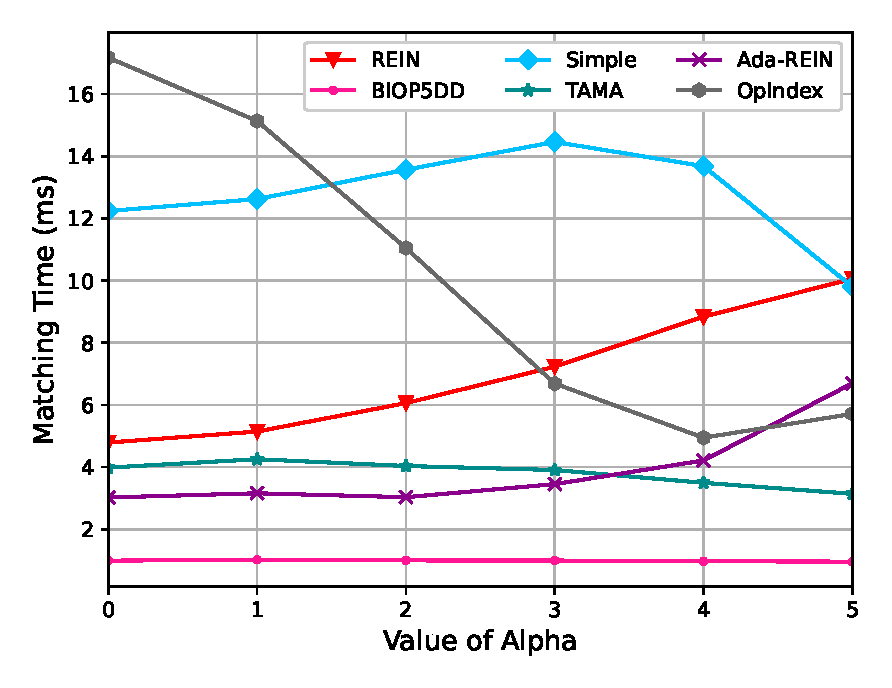
\includegraphics[width=5cm]{figures/exp8_alpha.eps}
\caption{Effect of $\alpha$}
\label{exp8}
\end{minipage}
\end{figure}


\subsubsection{Attribute Distribution.}
There are two categories of the skewed distribution of algorithm input. One is the value distribution and the other is attribute distribution. Considering that the matching time basically keeps invariant with an uneven value distribution of subscriptions and events, we only give the experiment results under skewed attribute distribution of both subscriptions and events in Fig. \ref{exp8}, where $d=50, \psi_S=5$ and $w=0.5$. In Zipf distribution, a larger $\alpha$ means a more serious skewed distribution and a more heavy workload. HEM and TAMA overcomes the skewed problem well while the other three counterparts fluctuate greatly with $\alpha$. Ada-REIN skips from 1 attribute and about 26 k predicates to 40 attributes and about 5M predicates when $\alpha$ varies from 1 to 5. Thus its matching time is smaller than that of REIN. 
%Note that the event attribute distribution is identical to the predicate distribution. Therefore, the substantially dropping matching times of OpIndex are attributed to the decreasing total number of predicates defined on pivot attributes, which lessens from 7.0 m to 1.5 m when $\alpha$ increases from 0 to 5. 

% \subsubsection{Comprehensive Experiment}
% % 缺少删除
% \vspace{-0.5cm} 
% \begin{figure}[htbp]
% \centering
% 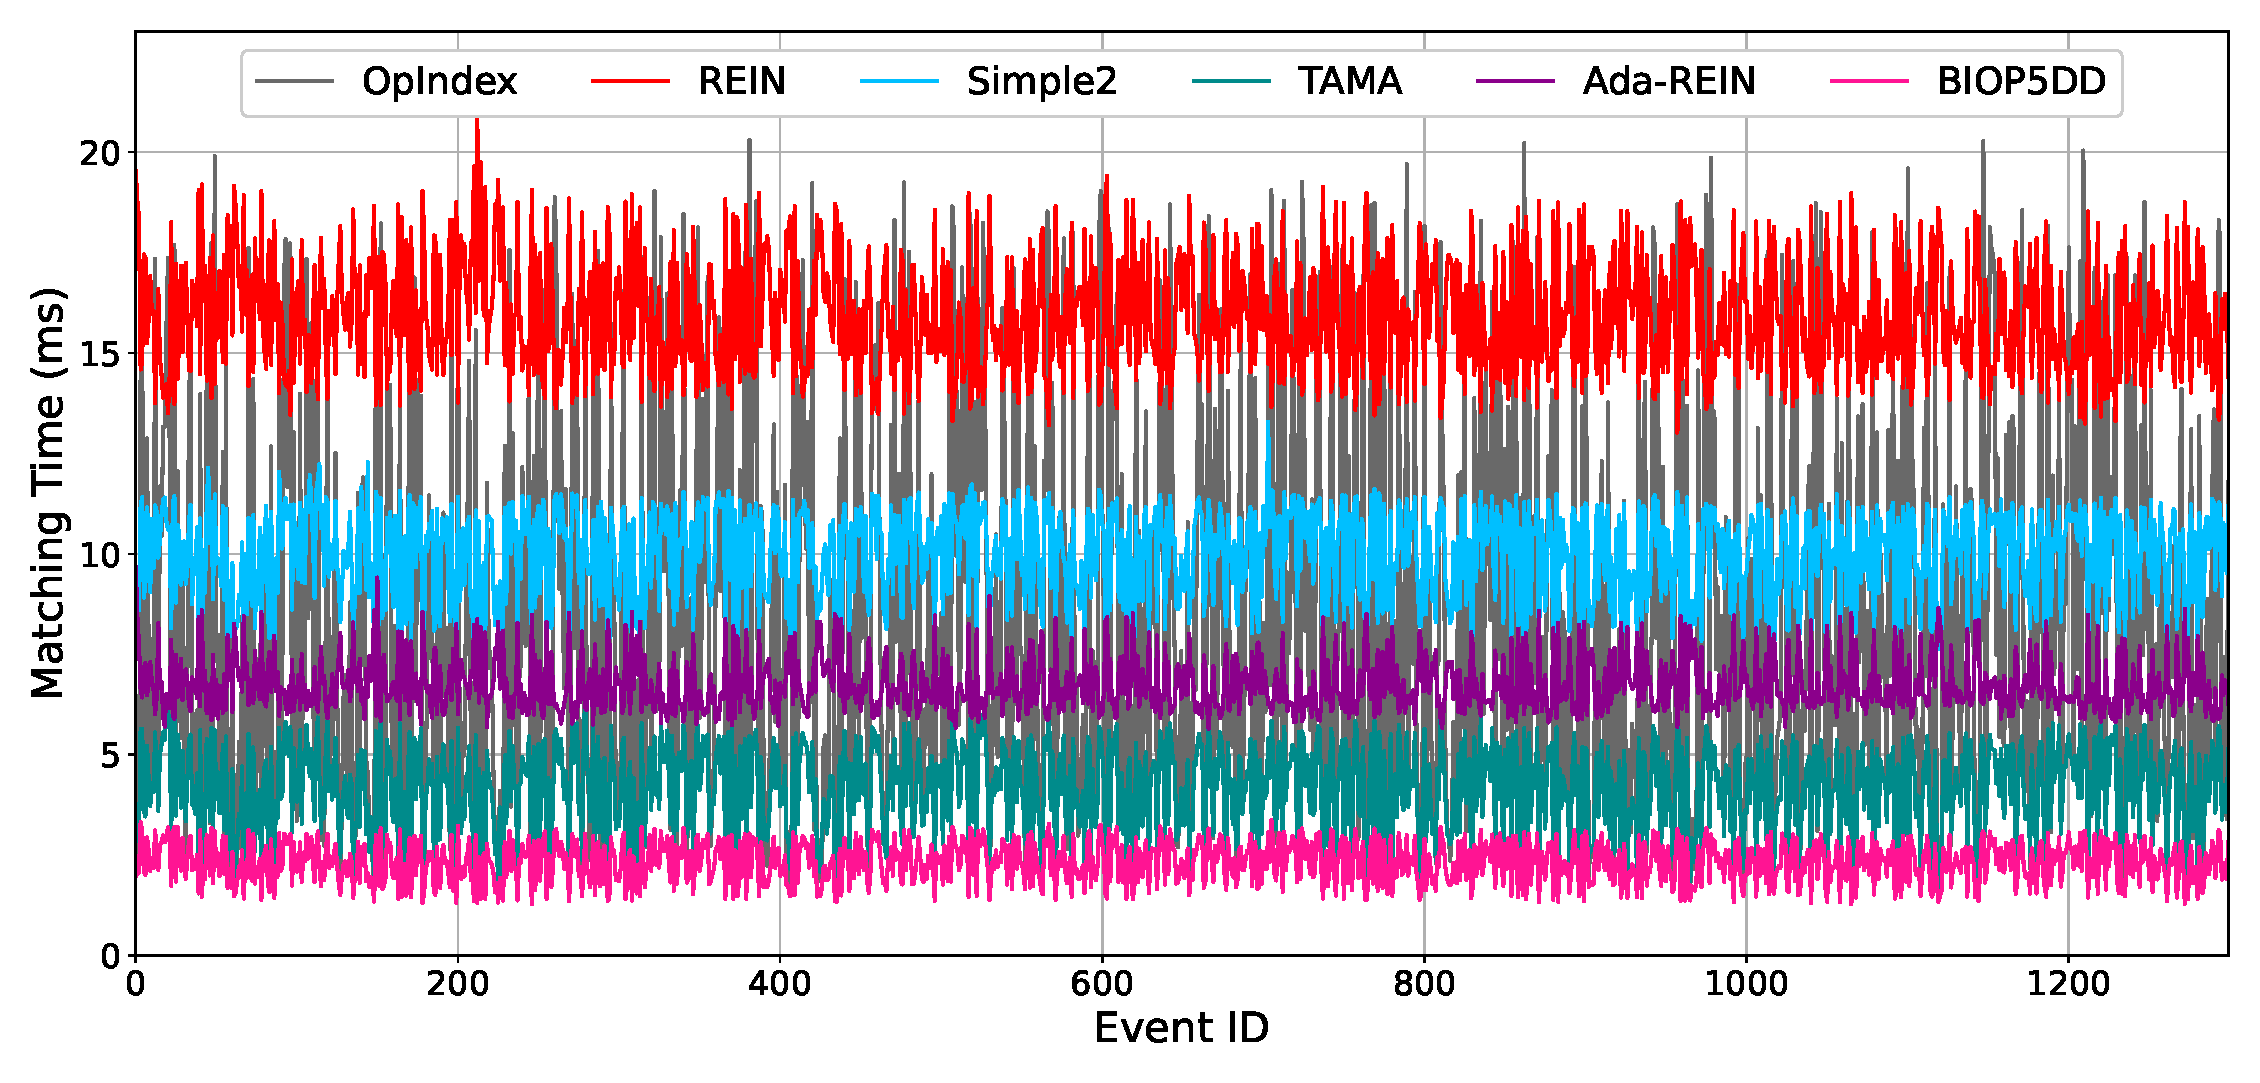
\includegraphics[width=11cm]{figures/exp9_comprehensive.eps}
% \caption{Exp9: Matching Time under Random Circumstance}
% \label{Exp9}
% \end{figure}

% Overall, HEM exhibits a superlative performance in matching time and stability under environments with a single variable. In Exp 4-6 and 8, the matching time of HEM changes a little compared to the other five methods. This is mainly due to the stable workloads of comparing tasks, bit or operations and counting tasks. To investigate the performance under dynamic workloads, we design a comprehensive experiment. In Experiment 9, $d=100, \psi_S=1\sim 20,\psi_E=1\sim40,w=0\sim1$. Parameters $\psi_S, \psi_E,w$ are randomly generated and attributes of predicates and events obey Zipf distribution with $\alpha=1$. Fig. \ref{Exp9} depicts 1300 event matching times of six algorithms. The results illustrates that HEM still has the lowest matching time. The relationship between the magnitude of the change in the matching time of the six algorithms is: $HEM5DD\textless $Ada-REIN$\textless$ Simple2$\approx$ TAMA$\textless$ OpIndex. In conclusion, HEM outperforms the five counterparts with respect to the matching time and robustness under extensive conditions.

\subsection{Maintainability}
% 构建时间、删除时间、内存
Two experiments are conducted to test the maintenance cost of HEM.
% Since the insertion time of HEM is essentially determined by $\psi_S$, we vary $\psi_S$ from 5 to 30 in the experiment.
Fig. \ref{istps} reveals that the average insertion time of HEM increases by about 42.6\% compared to REIN because HEM needs to pre-mark a new subscription in one or more bitsets for each attribute on which the predicate is defined.
TAMA inserts the subscription ID into a set of cells for each predicate, thereby resulting in the highest insertion time.
The deleting time of HEM is very close to that of REIN because the time to find the deleted pairs in cells accounts a lot. The experiment results are omitted.
Fig. \ref{Exp11} shows the memory usage of the five algorithms with different $n$. 
All the curves rise logarithmically. The memory usage of HEM is about twice of REIN's and 64.3\% of TAMA's.

\begin{figure}[tbp]
\centering
\begin{minipage}[t]{0.48\textwidth}
\centering
 \includegraphics[width=5cm]{figures/exp10_construction.eps}
\caption{Insertion time $\psi_S$}
\label{istps}
\end{minipage}% \quad
\begin{minipage}[t]{0.48\textwidth}
\centering
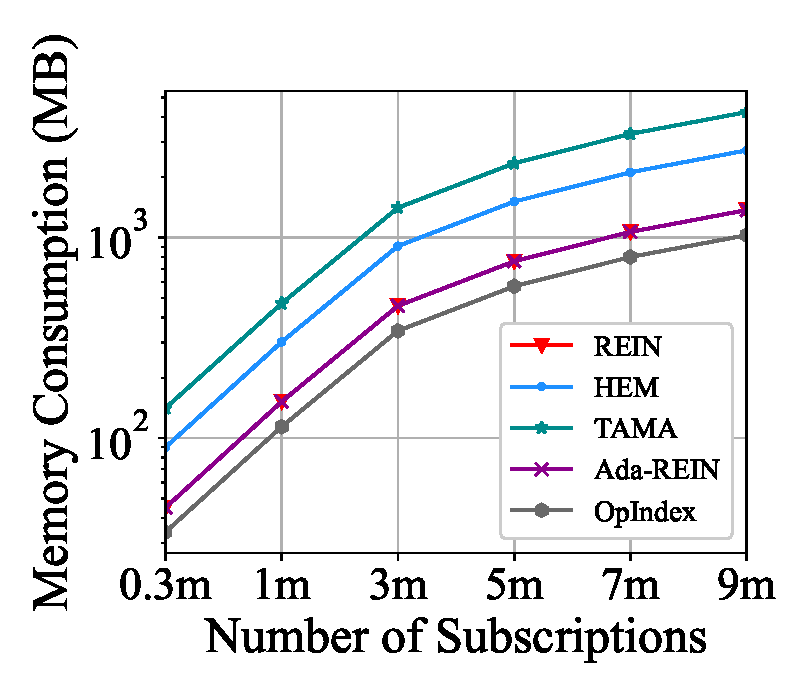
\includegraphics[width=5cm]{figures/exp11_memory.eps}
\caption{Memory usage(MB) by $n$}
\label{Exp11}
\end{minipage}
\end{figure}



% The deleting time curve by $\psi_S$ in millisecond is shown in Fig. \ref{exp10d}. Compared to respective inserting time, the deleting time of HEM, REIN, Ada-REIN, TAMA and OpIndex increases by about 83, 103, 112, 1.2 k and 29 k times when $\psi_S$ is 20. HEM behaves just a little worse than REIN. This is attributed to the stable and small workload to maintain the bitsets when $\psi_S$ is given.  
%When $\psi_S$ is 30,  the number of pivot attributes of OpIndex is 30 due to the uniform distribution, thereby reducing the number of predicates inserted into each pivot attribute index. Note that the average workload to find predicate pairs to be deleted is proportional to the number of predicates. Consequently, its deleting time obtains a little descent.
% instant
% The deletion operation for Simple is not relevant to $\psi_S$ because it checks the subscription ID one by one in the subscription list.

% \begin{figure}[htbp]
% \centering
% 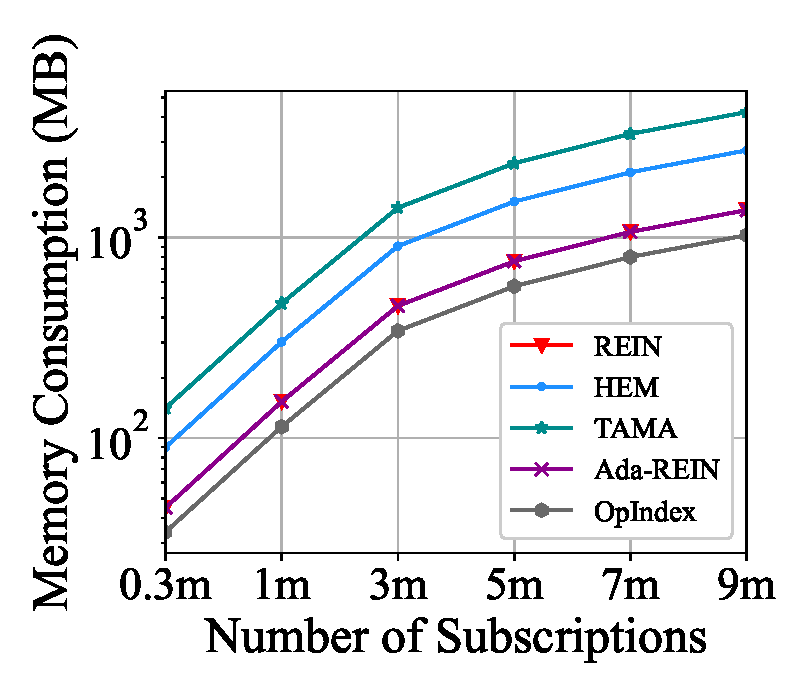
\includegraphics[width=5cm]{figures/exp11_memory.eps}
% \caption{Exp11: Memory Cost (MB) by $n$}
% \label{Exp11}
% \end{figure}

% The memory consumption is bound with $n, \psi_S,$ and $d$. 


\section{Conclusion}
\label{co}
When processing a large number of subscriptions, most matching algorithms need to repeatedly perform a lot of operations, which becomes a performance bottleneck.
% Millions of bitwise OR instructions parallelly operated on bitsets are faster than one bit operation one time. 
In this paper, we propose a hardware-aware event matching algorithm termed HEM, aiming to execute efficient operations in the matching process. The experiment results reveal the superiority of HEM to its counterparts. 
HEM shows excellent performance in terms of matching time and stability under various conditions. 
In the future, we plan to design a state reduction method to optimize the bit OR operations of HEM under high dimension, and extend HEM to multi levels to accommodate input with multiple hotspots.
% Two optimizations (DRO and DPO) are put forward to strengthen the mnemonic and perceptual ability of original HEM. 
% 1. HEMSC: various standards to classification
% 2. HEMSR and its maintain
% 3. Threashold $t$.
%引入阈值参数 t,在一个维度上谓词个数达到 t 后才开始用bitset,适合高维的情况,因为高维空间下谓词很稀疏,一个维度上可能没几个谓词,很多空桶,遍历一遍可能比或运算快
% 4. The number of bitset can be equal to $c$. 

\section*{Acknowledgments}
This work was supported by the National Key Research and Development Program of China (2019YFB1704400), the National Natural Science Foundation of China (61772334, 61702151), and the Special Fund for Scientific Instruments of the National Natural Science Foundation of China (61827810).



\bibliographystyle{splncs04}
\bibliography{sample-base.bib}
\end{document}
